% !TEX program = lualatex

%      File: VTthesis_template.tex
%     Created: Thu Mar 24 11:00 AM 2016 EDT
%     Last Change: Thursday, December 19, 2019
%     Author: Alan M. Lattimer, VT
%	  With modifications by Carrie Cross, Robert Browder, and LianTze Lim. 
%     modifications by Ziling Wu, PhD, Electrical and Computer Engineering department, VT, 2016-2020
% This template is designed to operate with XeLaTeX.
%
% All elements in the Title, Abstract, and Keywords MUST be formatted as text and NOT as math.
%
%Further instructions for using this template are embedded in the document. Additionally, there are comments at the end of the file that give suggestions on writing your thesis.  
%
%In addition to the standard formatting options, the following options are defined for the VTthesis class: proposal, prelim, doublespace, draft. 

\documentclass[doublespace,nopageskip]{VTthesis} % nopageskip - Removes arbitrary blank pages.

% Using the following header instead will create a draft copy of your thesis
%\documentclass[doublespace,draft]{VTthesis}

% The lipsum package is just included to put dummy text in the document in order to demonstrate page headers and table of contents behavior. You should remove it once you begin writing your actual thesis or dissertation.
\usepackage{lipsum}
\usepackage{todonotes}
\usepackage[numbers]{natbib}
\usepackage{xparse}
\usepackage{multirow}
\usepackage{dirtytalk}
\usepackage{listofitems}
\usepackage{numprint}
\usepackage{siunitx}
\usepackage{array}
\usepackage{pdfpages}
\usepackage{unicode-math}
\usepackage{float}
% \setuptodonotes{textwidth=0.5}

\setlength{\marginparwidth}{2cm}
\NewDocumentCommand{\rtodo}{O{} m}{\todo[author=Richard #1]{#2}}
\NewDocumentCommand{\vstodo}{O{} m}{\todo[author=Vivek #1]{#2}}

% Title of your thesis
\title{Modeling Expressive Musical Performance with Transformers: An Empirical Error Study}
% \title{Modeling Expressive Musical Performance with Transformers: An Empirical Error Study}
% \title{Modeling Expressive Musical Performance with Transformers}

% You should include 3-5 keywords, separated by commas
\keywords{Some Keywords, Subject matter, etc.}

% Your name, including middle initial(s)
\author{Richard W Timpson}

% Change this to your program, e.g. Physics, Civil Engineering, etc.
\program{Your Department} 

% Change this to your degree, e.g. Master of Science, Master of Art, etc.
\degree{Doctor of Philosophy} 

% This should be your defense date:
\submitdate{December 4, 2020} 

% Committee members. Only have five readers and one chair available.
% Only use the ones you need and don't include the ones you don't need.
% You can also declare a Co-advisor. If you do, the principal and co-advisors
% will be listed as co-advisors on the title page.  Per the VT ETD standards, 
% you should not include titles or educational qualifications such as PhD or Dr.
% You should, however, include middle initials if possible.
\principaladvisor{Your Advisor}
%\coadvisor{Vicente Esparza}
\firstreader{First Committee}
\secondreader{Second Committee}
\thirdreader{Third Committee}
\fourthreader{Last Committee}

% The dedication and acknowledgement pages are optional. Comment them out to remove them.
\acknowledge{I would first like to acknowledge Professor Srikumar for agreeing to take me as his student and advise me in my research. When I first approached him with the general idea of doing a research project involving Machine Learning and music, neither he nor I had the slightest bit of background in the research area. Although this project's scope has been relatively small, we have both learned an immense amount about music information retrieval and broadened our scope of understanding in applied Machine Learning, which had previously centered around NLP. I want to thank Vivek for his efforts in supporting me in my research interests even though he had limited domain knowledge. 

I would also like to thank my wife Vivian and my daughter Sonya for understanding and supporting me through some of the struggles that I encountered while working on this project. The last six months have been a chaotic time for both my family and me, and without their continued support, I would not have been able to complete the project on time. I look forward to giving them more of my attention and time now that it is complete. }
 

% The abstract is required.
\abstract{Give a brief description of your thesis here.}
\abstract{%%% -*-LaTeX-*-
%%% This is the abstract for the thesis.
%%% It is included in the top-level LaTeX file with
%%%
%%%    \preface    {abstract} {Abstract}
%%%
%%% The first argument is the basename of this file, and the
%%% second is the title for this page, which is thus not
%%% included here.
%%%
%%% The text of this file should be about 350 words or less.

Here is an abstract. 
}

\graphicspath{{tex/figs/}}



% The general audience abstract is required. There are currently no word limits.
% \defaultfontfeatures{Scale=MatchLowercase}

\begin{document}
% The following lines set up the front matter of your thesis or dissertation and are required to ensure proper formatting per the VT ETD standards. 
  \frontmatter
  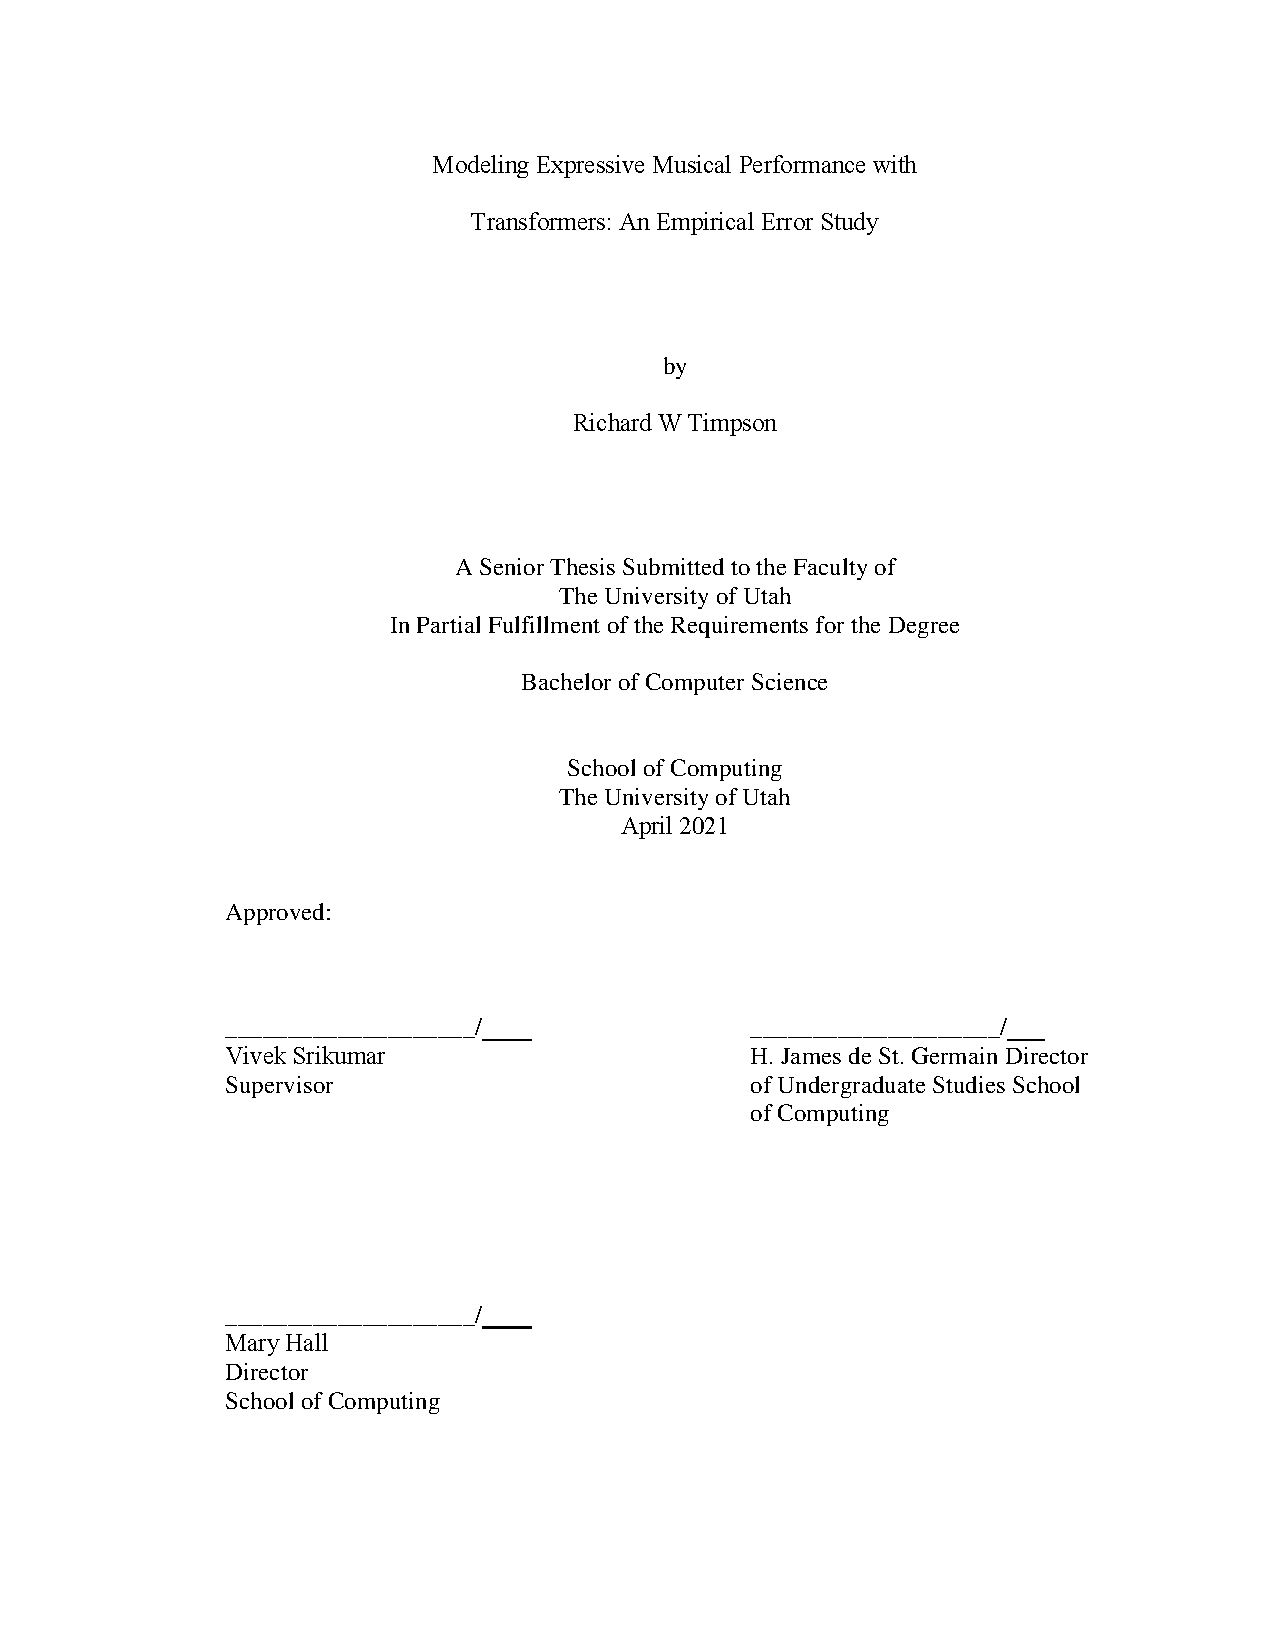
\includepdf[pages=-]{contents/SampleCoverPage.pdf}
  \maketitle
  \tableofcontents

% The list of figures and tables are now optional per the official ETD standards.  Unless you have a very good reason for removing them, you should leave these lists in the document. Comment them out to remove them.
	\listoffigures
	\listoftables
	% % sample text for abbreviations:
\nomenclature{NLP}{Natural Language Processing}
 
\nomenclature{$\sigma$}{The total mass of angels per unit area} 
    % \printnomenclature %Creates a list of abbreviations. Comment out to remove it. 

% The following sets up the document for the main part of the thesis or dissertation. Do not comment out or remove this line.
	\mainmatter

	% Adding table macros here that are used in various different sections
	% model configuration
	\newcommand{\nep}{$N_{id}$}
	\newcommand{\mn}{$M$} % mn for 'model name'
	\newcommand{\nl}{$L$} % nl: num layers
	\newcommand{\dhid}{$d_{hid}$} % dhid: dimension hidden size
	\newcommand{\drop}{$D$} % D: Dropout
	\newcommand{\lr}{$LR$} % LR: Learning Rate
	\newcommand{\clip}{$C$} % C: gradient clip
	\newcommand{\nh}{$H$} % nh: num heads

	% Expressive features
	\newcommand{\temp}{$t$}
	\newcommand{\vel}{$v$}
	\newcommand{\dev}{$d$}
	\newcommand{\art}{$a$}
	\newcommand{\ped}{$p$}

	\newcommand{\tm}[1]{$T_{N_{#1}}$}

	\pagestyle{headings}
	%now go ahead and start writing your thesis
	\chapter{Introduction} \label{ch:introduction}

% In 1952 L.A. Hiller and L.M Issacson ushered forth a new era of the study of both music and computer science when they introduced the Illiac Suite – the first composition that was created solely by a computer \cite{sandred2009revisiting}. What we'll refer to broadly as Computer Music (CM) research has continued to see impressive advancements since the introduction of the Illiac Suite in several different domains, including musical composition\cite{briot2017deep}, instrument and sound synthesis\cite{engel2017neural}, and musical analysis\cite{widmer2016getting}. CM research presents a unique challenge to both musicology and computer science due to the highly subjective nature of music paired with the strong quantitative and mathematical nature of computer science. However, music is also inherently mathematical and contains a strong hierarchical structure from which powerful patterns emerge - how it is that these common patterns lead to such a highly subjective human experience is outside of the scope of this work. It is perhaps due to the inherently paradoxical nature of music that it creates such an interesting set of problems to study, particularly from a computational perspective. In the authors opinion, this problem set is one of the most worthwhile to study in the current day, and should receive more focus in the research literature. 

% To reach such a point, it is necessary to view the field from the lens of Artificially Intelligent musical systems that are able to reason themselves about music. In general, Artificially Intelligent systems have seen immense progress in the last decade due to the rise of Machine Learning (particularly with Deep Learning) and it's applications in several different domains. Music has been one of these domains and has seen impressive advances in several musical tasks such as musical composition\cite{huang2018music}, and musical analysis\cite{widmer2016getting}. 

% One of the more intriguing problems in computer music is the creation of an expressive performance generation system. There are several commercially available notation and playback software systems \footnote{\url{musescore.com} and \url{www.finalemusic.com}} that are able to automatically generate musical performances from a purely symbolic musical representation in the form of a score (more commonly known as sheet music). The systems are built based on a predefined set of rules that create deterministic performances given a score. Although the performances are technically an "accurate" rendering of the score, they don't contain the \emph{human} element. That is, they contain a straight and deterministic mapping between a note marked in a score and its corresponding position in the associated performance. In such systems, there is no \emph{expression} of the performance. As such, these systems produce robotic-sounding performances that are offputting to human listeners \footnote{an example performance can be heard from \href{https://musescore.com/user/33884420/scores/6466906}{musescore}}. 

% These simple performance generation systems do not render "expressive" because they don't account for performance features that add the human element. Such features include variations in tempo, timing, and dynamics (TODO: Add a reference to a later section that will go over each feature in detail). A performer of a composition uses each of these features of the performance to add a unique interpretation of the piece. This interpretation (or expression) is responsible for providing the "human" element of musical performance. 

% This poses the question of whether or not a computer system can create expressive performances that are close to actual human performance (or even creating a completely new style of expression that a human cannot). This has been an active area of computer music research since the 1980s \cite{friberg2006overview}. This thesis is a further exploration of the current research with a particular emphasis on applying the current state of the art Deep Neural Network architectures from Natural Language Processing (NLP) research to the problem domain and understanding their effects. \rtodo{Revisit introduction after outline and more writing}

\begin{itemize}
    \item Introduce the idea of musical research with computers. Talk about the illiac suite \cite{sandred2009revisiting} and Music Information Retrieval.
    \item Significance of machine learning on the field 
    \item Introduce idea of expressive musical performance. Brief conversation about the different performance components (articulation, dynamics, timing). 
    \item Using Transformer architecture which hasn't been done in the field. 
    \item \rtodo[,inline]{report results}
\end{itemize}
	\chapter{Background: Expressive Performance}\label{ch:ch2}
This project is based upon two major research components. The first is the MIR problem domain of expressive musical performance, and the second is the modeling domain of Transformers. In this chapter, we will introduce and discuss EMP. In chapter \ref{ch:ch3} we'll do the same for the Transformer. 

Expressive musical performance is a small subset of Music Information Retrieval research, which we broadly categorized into two separate tasks: the first is developing computational methods for musical analysis, the second is developing computational methods for music generation. We are interested in generative models, although it is worthwhile to note that there is considerable overlap between the two areas\footnote{Creating a performance generation system is useful for performance analysis as long as the generation system is interpretable. The reverse is also true. Analysis provides insight to generation, and generation provides insight to analysis}. A proper knowledge of the entire musical generation process as a whole is necessary to understand how EMP generation models work. \citet{ji2020comprehensive} break the generation process into three stages with four different roles that interact with that process at each stage. Figure \ref{fig:generation_process} shows each step in the process as well as the agents that participate. 

\begin{figure}
    \centering
    \missingfigure{Image that shows different components of musical generation process}
    \caption{The first step of musical generation is composition, shown as a score in the figure. The second is performance, which is our area of interest. The third is the production of sound. Each different agent: composer, performer, instrument, and listener, can be thought of as a separate computational model in the generation process}
    \label{fig:generation_process}
\end{figure}

An EMP generation model is analogous to the performer shown in \ref{fig:generation_process}, who takes as input a composition and produces as output a performance. We define musical expression as the performers' interpretation of a composition codified into different performance parameters intended to contribute to the quality of a musical experience% 
\footnote{As has already been mentioned and as will show in detail later in this work, defining the ``quality'' of musical experience is no minor task. Such a definition is necessary to train performers (either computer or human) to create desirable performance.}. 

Figure \ref{fig:generation_process} shows that a performer interacts with a composed score to create a performance. To more clearly define EMP generation, we start by describing the essential elements of both scores and performances. This chapter's descriptions are not intended to be at a detailed mathematical level but the general musicological level. We provide feature definitions, which contain the score and performance information embedded at a mathematical level and are necessary for building any computational model, of some of the EMP models upon which our work is based in section \ref{sec:emp_generation_models}. We refer the reader to appendix \ref{ase:app_one_sect_1} which provides some basic musical terminology and concepts that will be useful for understanding our definitions\footnote{Most of the appendix material may seem elementary to those who already have a background in music or musical notation}. Due to the constraint of our data, we focus only on western classical piano music. 

\section{Scores}\label{sec:scores}
Scores are symbolic representations of a musical composition. They are expressed through a language of symbolic notation used to express musical ideas and information. Scores present this information in a hierarchical structure with different levels of musical detail at each level. Figure \ref{fig:score_hierarchy} shows a sample score and the different hierarchical levels of information that it contains

\begin{figure}
    \centering
    \missingfigure{Image that shows a sample score with colorized annotations that show the different hierarchical levels}
    \caption{Caption will be dependent on the image.}
    \label{fig:score_hierarchy}
\end{figure}

%mnot for musical notation. Bold and emphasize at once
\newcommand{\mnot}[1]{\textbf{\emph{#1}}}

The lowest level contains information about the pitch and timing of every single note, as well as optional information about how the note should be played. This can include information specific to instruments such as the bow direction of a violin, but for our purposes (dealing only with piano) we will consider this to be the articulation of each note, usually indicated by \mnot{legato} or \mnot{staccato} \rtodo[,inline]{Make sure to have some background information on articulation in the appendix}

The middle level contains information related to certain substructures within the musical composition, which are usually expressed within a grouping of notes or measures. The most common score annotations at this level are dynamic markings which indicate whether to play a grouping of notes as \mnot{f} (loud), \mnot{p} (soft), or as a \mnot{crescendo} or \mnot{decrescendo} (gradually increase or decrease the volume). %\rtodo{Add correct notation markings) %
Although dynamic markings are the most common at this level, it is also possible to see score markings for all other musical features, such as local tempo or articulation of a certain substructure. Perhaps the most important score marking at this level is that of a phrase, which is a marking that indicates that a group of notes should be interpreted as belonging to a singular musical idea and that each note should fit within the context of the phrase as a whole. A phrase can be expressed through all of the different aforementioned musical features, including the tempo, timing, dynamics, and articulation of the notes.

The highest level contains meta-information that relates to the entire composition as a whole. This information typically includes the key signature and time signature, as well as the global tempo for the entire piece, most commonly represented as BPM. 

% \subsection{Score Features}
% \rtodo[,inline]{This entire section needs work. Include some detailed information but refer reader to chacon's thesis for a full breakdown. Possibly mention features from virtusoNet}.

% There are some score features which are required for EMP models, which include the musical features at the lowest level of a score as explained in section \ref{sec:scores}. These are pitch and timing, and the duration of the notes. Mid-level features include concepts at the local level and have some music theoretic concepts, such as downbeat information of a given measure according to the time signature, or the tonality of a chord (tonic, dominant, etc). High-level features represent advanced music theoritic concepts that are more global to the entire piece, including abstract properties of the piece such as the emotion the piece should convey and how different sections of the piece relate to each to tell a complete story \cite{eduardo2018computational}. 

% Both the mid-level and high-level features are not necessarily required for every EMP model as the lower-level features are, and are not consistent across all EMP models. It still remains an open question as to which features should be extracted from the data that the model can learn from. The lack of consistency in these features is one of the reasons that evaluation of EMP generation models is so difficult, as explained in section \ref{sec:evaluation}. 


\section{Peformance}\label{sec:performance}
An expressive musical performance contains most of the same musical information as does a score, including pitch, tempo, timing, and articulation. However, there is one key difference between the two. Expressive performances will deviate (or interpret) from the exact information given in the score. For example, although a score may indicate a tempo of 120 BPM, it is unlikely that a given performer will perfectly adhere to this tempo throughout the piece's entirety. This interpretation is even more apparent if the score indicates a change in tempo somewhere in the composition. If a score contains an \mnot{accelerando}, meaning that the performance should speed up over a series of notes, there is no precise indication of the rate at which the tempo should increase. Some performers may choose to speed up at a fast pace and over a short period. Others may decide to increase the tempo at a slow rate and over a more extended time period. A single \mnot{accelerando} can ``correctly'' result in either of these outcomes. 

Each expressive parameter will be measurable and absolute, whereas the score markings of these features are more of a suggestion than a rule. Performance has a few additional components that are not necessarily indicated in scores but are relevant in the context of performance alone. The first we will refer to as deviation, which is heavily related to timing. It is represented as a numerical number that represents how far off the timing of a particular note deviates from its ``correct'' position in the score. These micro-timing deviations present in musical performances are an essential part of expression. Without them, each note onset and offset would fall precisely in line with its marking in the score. This is how current commercial EMP generation systems operate, resulting in performances that are deterministic, robotic, and mundane \rtodo[,inline]{add a reference, graphic, and sample performance}. 

Pedaling in piano performance is another important feature of performance that is not always present in a score. There are several different types of piano pedals. The most common are the sustain pedal, which prolongs every notes' duration when activated, and the soft pedal, which softens the entire piano's sound. Although these pedals' effects are directly related to the articulation and dynamics of the performance, their presence (or lack of) is a crucial component of piano performance. The sustain pedal is actively used in almost all modern piano performance, even in the absence of pedal score markings. 

% \subsection{Performance Features}
% \rtodo[,inline]{Similarly to score features section, provide more detailed information about some of the math behind the features. Cite other resources where necessary}
% For western classical solo piano music, performance features are relatively simple compared to the score features as well as to other instruments. Most EMP models use the different aspects of a piano performance as explained in section \ref{sec:performance} for their data features, including the pitch, tempo, timing (or timing deviation), articulation, and pedal. Although at an abstract level the features are the same, there are different numerical methods used to describe each of the different aspects. These are presented in \rtodo[,inline]{Add reference to relevant work section that goes over the different elements. This information may belong better here and then referenced in the relevant work section}. 

\section{Data}
The data required for EMP generation includes a digital representation of a score and a corresponding performance. MusicXML, a text-based representation of a composition, is the most common data format for a score. Performances could directly be represented through raw audio, which is widely available on the internet. Instead of audio however, an intermediate data form, MIDI, is commonly used to constitute the performance. MIDI is an event-based data format and software interface that contains information about different aspects of a recorded performance. This information includes the recorded timing, pitch, and volume of every note, the instrument used, and pedal information (specifically in the case of piano performance). 

There are several reasons for the preference of MIDI over raw audio. The first is that audio data is inherently noisy, sparse, and larger in its dimensionality and size. Using audio to represent performance requires a significant compression of natural frequencies into more abstract musical representations such as pitch -- MIDI natively contains these abstractions. MIDI also better aligns with the generation process outlined in \ref{fig:generation_process} in which performance is seen separate from sound synthesis and allows computational models to define such boundaries easily. In the full generation process, a different model would be used to take the performance data in MIDI and synthesize it into raw audio presented to the listener. 

Both MIDI and MusicXML contain all of the required information to represent all of the musical components of both a score and a performance, including pitch, tempo, timing, articulation, deviation, and pedal. See appendix \ref{ase:app_one_sect_2} for more information on both MusicXML and MIDI. 

Computational models that deal with the relationship between scores and performances often need additional metadata about the alignment between every note in both the score and performance. This metadata is generated by running a performance and its corresponding score through a data alignment process in which every performance is matched to a marking in the score. Given the highly dynamic nature of musical performance, it is a non-trivial task to run this alignment process for a set of scores and performances, especially if the task is performed by manual human annotation. There exist methods for both manual and automatic alignment. Due to the time-consuming nature of manual alignment and the need for large data sets to build higher quality models, automatic alignment algorithms are an active area of research.

\begin{figure}
    \centering
    \missingfigure{Show why score to performance alignment matching is necessary.}
    \caption{Two performances of the same score can vary wildly in their tempo and timing. This makes it necessary to have a score to performance alignment for every performance. }
    \label{fig:alignemnt}
\end{figure}

\subsection{Existing Data Sets}
\rtodo[,inline]{Rework this section to fit with new paper outline. Need to forward reference models instead of back reference}
One of the problems facing EMP and MIR is the lack of high-quality and large-scale datasets\cite{cancino2018computational}. The broad scope and diversity of data across the different musical components partly explain this absence. As has been discussed, there are different stages in the musical process, and there are different ways to represent music at each stage. For example, composition can contain the same amount of information in at least three forms. The first and most common is the symbolic representation in the form of a data format like MusicXML. As we have seen, we can infer much of the information necessary to construct a score from performance alone, given that performance contains the timing and pitch of every note. Such score information is naturally embedded in both MIDI and raw audio. 

The biggest hindrance in data gathering is that most of the musical data available on the internet is in the form of audio. As we have pointed out, processing audio data for musically plausible purposes is difficult compared to other better-suited formats. While a fair amount of MusicXML and MIDI does exist, it is relatively small compared to the amount of audio data. We draw a comparison to the data used in NLP research, where textual data is analogous to MusicXML and MIDI, and speech audio is analogous to musical audio. One of the reasons NLP has been able to significantly advance its progress in the last few decades is because of the massive amount of readily available textual data on the internet. If NLP only had available text data as represented by audio, as is often the case with music, it would be significantly more challenging to develop NLP systems and applications. Nevertheless, there has been a recent effort to gather quality data in MIR. We present some of these datasets as they are relevant to EMP. 

There are normally 3 required components for a EMP dataset. 
\begin{enumerate}
    \item Scores (usually in the form of MusicXML)
    \item Performances (usually in the form of MIDI)
    \item Metadata about the matching alignment between the score and performance. 
\end{enumerate}
Score data can be gathered by finding readily available MusicXML files from open source software projects which contain music that is in the public domain (which all western classical music is) \footnote{\href{https://musescore.com}{MuseScore} is the most common. Also see the \href{https://imslp.org/wiki/Main_Page}{International Music Score Library Project}}, or by using Optical Music Recognition (OMR) to automatically scan paper sheet music into a digital form followed by manual corrections where needed. MIDI performances can only be recorded when a performer uses an instrument that is compatible with the MIDI protocol. Although there are many digital piano keyboards with this combability, semi-professional and professional pianists primarily play on acoustic pianos. Some computer-controlled acoustic pianos can record MIDI performance, such as the Yamaha Disklavier and the older Bosendorfer CEUS system. Therefore, MIDI data of professional piano performance has historically been limited to performances on these piano systems. 

There is no standardized method for score-to-performance alignment methods and data representations. Each dataset presents its own alignment method as well as the metadata that represents the alignment. 

To provide context for the progression of data used in EMP generation, we will introduce an older dataset used in EMP research, the Magaloff Corpus. We then describe a much larger scale dataset, the Piano-e-competition, which has recently been adapted for EMP generation use.~\citet{cancino2018computational} give a full overview of datasets used in EMP generation. 

\subsubsection{Magaloff Corpus}
Nikita Magaloff was a Russian pianist known for his performance cycles of Chopin's entire works for the solo piano. In one of his final cycles of performances recorded in 1989, he played on a Bosendorfer SE computer-controlled piano.~\citet{flossmann2010magaloff} obtained special permission to access the MIDI data from this performance cycle. They gathered score data using OMR with manual corrections where needed.  The alignment method of~\citet{grachten2006expressivity} was used to produce the note-matching annotations, along with manual corrections. The dataset contains over 10 hours of playing, 150 compositions, and over 320,000 performed notes. The corpus, however, is not publicly available and has only been used in research by \citet{flossmann2010magaloff} and colleagues \cite{eduardo2018computational}. 

\subsubsection{Piano-e-competition}
As has been discussed, there is a large push in modern MIR to produce high-quality large datasets. At the heart of this research in MIR is the Piano-e-competition. Started in 2002, it is an international piano competition which attracts some of the promising up and coming musicians at both the senior and junior level \cite{the-disklavier-education-network}. Every performance from the competition is played on a Yamaha Disklavier and is recorded in both MIDI and audio. Due to the data set's size and availability, it is commonly used in MIR research. There exist several different adaptations of the original data that are specific to particular research purposes. 

The first of these is the MAESTRO (Midi and Audio Edited for Synchronous TRacks and Organization) dataset. \citet{hawthorne2018enabling} introduce the MAESTRO dataset, which presents both MIDI and audio data from the Piano-e-competition in a canonical and easily accessible form. The dataset was first used to build a full musical analysis and generation process framework named wav2midi2wave. This framework includes a musical transcription process \cite{hawthorne2017onsets} from raw audio to midi (wav2midi), a direct musical composition and performance generation model \cite{huang2018music} \footnote{This model directly generates MIDI files without using scores. It simultaneously generates a composition and performance. This direct generation is a merging of the two separate tasks into one as shown in figure \ref{fig:generation_process}} (can be seen as the midi or midi2midi part of the wav2midi2wav framework), and a synthesis model that takes MIDI and generates raw audio\cite{oord2016wavenet} (midi2wav). The MAESTRO dataset is the most commonly used form of the Piano-e-competition data. 

The Piano-e-competition also forms the basis for a data collection, which we will refer to as the KAIST dataset\footnote{We take the name from the KAIST Graduate School of Technology, which the researchers who created the dataset work for}. The Piano-e-competition dataset itself does not provide any score data about any of the compositions used in performance. The KAIST dataset was created specifically for an EMP generation system, and therefore needs score data for every performance recorded in MIDI. This score data was collected by \citet{jeong2019virtuosonet} by downloading MusicXML files online, mostly from MuseScore. On top of gathering the score data for all performances in the Piano-e-competition, \citet{jeong2019virtuosonet} also run the automatic score-to-performance alignment algorithm of \citet{nakamura2017performance} to provide metadata about the alignment between each score and performance. Automatic score-to-performance alignment is error-prone, especially in the case of performance mistakes\footnote{A mistake in the performance results in a performance note having no correct match with a score note.} As a result, some performance notes are not aligned to those in a score. Due to the possibility for error in automatic alignment, \citet{jeong2019virtuosonet} also add additional manual and heuristic corrections to the alignment where needed. 

Other than the discrepancy in scale, the most significant difference between the KAIST dataset and the Magaloff corpus is that the KAIST dataset contains multiple performances for the same score. In contrast, the Magaloff Corpus has a 1-1 mapping between a score and performance. The KAIST dataset has 226 scores across 16 different composers, roughly 660,000 score notes, and around 3,500,000 performance notes. The number of matched performance notes is ten times larger than the Magaloff Corpus, and all data is publicly available \footnote{The dataset is open sourced at \url{https://github.com/mac-marg-pianist/chopin_cleaned}}. 

The Aligned Scores and Performances (ASAP) dataset~\cite{foscarin2020asap} is a recent adaptation of both the KAIST dataset and the MAESTRO dataset. It uses the MusicXML files from the KAIST dataset, audio from the MAESTRO dataset, and MIDI files from both sources extracted from the common origin of the Piano-e-competition. It provides additional alignment metadata for both MIDI and audio and more manual correction in the MusicXML score files. Although the purpose of the ASAP dataset is for Automatic Music Transcription (AMT)\footnote{AMT is the task of transcribing a score from a performance (either in audio or MIDI form). AMT is the "opposite" of EMP. It maps a performance to a score instead of a score to performance}, it is just as equally useful for EMP generation. To our knowledge, it hasn't seen an application in any EMP generation task. Although it is mostly similar to the KAIST dataset, the implications of its extensions are undetermined in EMP research. 


\section{Performance Evaluation}\label{sec:evaluation}
Evaluation is an essential component of developing ML models. A models' evaluation is a measure of its quality and serves as a benchmark that can be compared to other models in the same domain. Due to the inherently subjective nature of music and musical performance discussed in chapter \ref{ch:ch1}, evaluation is notoriously difficult to understand and define correctly for EMP generation models~\cite{cancino2018computational}. 

The evaluation of computational models, specifically for EMP models, is typically categorized in two ways: quantitative and qualitative evaluation. Quantitative evaluation methods involve using numerical metrics, which are computationally generated and deterministic. Qualitative evaluation methods usually involve human feedback and judgment, often presented in some standardized statistical measures. The key difference between quantitative and qualitative is that qualitative methods are not as consistent and more challenging to reproduce, given the reliance on human listeners' subjective feedback. Quantitative evaluation methods are traditionally preferred over qualitative because of their consistency and reliability. However, in the case of music generation models, qualitative evaluation methods may be more relevant because of music's highly subjective nature. Finding suitable methods of evaluation is an active area of research in EMP \cite{cancino2018computational}. 

\subsubsection{Quantitative Evaluation}
There are several different metrics commonly used in the evaluation process, all of which are specific to the type of data and problem domain the model fits inside. Our model is a regression model, which we cover in chapter \ref{ch:ch5}, and so we present some standard metrics used to evaluate regressive EMP models. 

The two common metrics used for evaluation and regression are Mean-Squared-Error (MSE) and the Coefficient of Determintation (commonly abbreiated as $R^2$). MSE is used to measure the difference between a prediction and an actual observed target value, and can be denoted as $MSE = \frac{1}{n}\sum_{i=1}^{n}(Y_i - \hat{Y_i})^2$, where $Y_i$ is the observed value at time step $i$, and $\hat{Y_1}$ is the predicted value. $R^2$ is a probablistic measure of the linear correlation between variables $X$ and $Y$, and is denoted as $\rho_{X,Y} = \frac{cov(X,Y)}{\sigma_{X}\sigma_{Y}}$ where cov indicates the covariance and $\sigma$ indicates the standard deviation.

\subsubsection{Qualitative}
Qualitative evaluation in EMP is most often conducted by presenting computationally generated performance to human listeners and gathering feedback and judgment. Although there have been efforts to standardize this evaluation process, the qualitative evaluation methods of different EMP models significantly vary. The lack of consistency in the evaluative methods makes reproducing experiment results difficult in EMP research, but it is still perhaps the best way to evaluate EMP models today. 

The most significant effort in EMP generation qualitative evaluation was the Performance Rendering Contest (Rencon)~\cite{katayose2012evaluating}. Starting in 2002 and ending sometime around 2013~\cite{cancino2018computational}, Rencon was an annually held competition that provided a way to compare EMP systems using standardized and evaluation methods. It did so by subjecting each models' performances to the same listening judges and judgment rubric, thus adding a higher level of confidence in each model's final quality judgment. 

Although the evaluation methods changed from year to year, they all followed the same general structure. To enter the competition, contestants would submit MIDI files of generated performances by their respective models. The choice for compositions was usually restricted to a small set of composers, such as Chopin or Mozart. A Yamaha Disklavier was then used to create an acoustic rendering of the generated MIDI file played in front of a set of judges. The judges' makeup usually included musical experts with varying experience. The judges submitted a feedback survey that would rate aspects of performance such as "rhythmic accuracy," "musical skill," and "overall quality," along some standard statistical scale. A winner was chosen according to the judge's survey entries. 

Although Rencon does not currently hold competitions, it forms the basis for many of the methods used in the qualitative evaluation of EMP models. As mentioned, the exact survey methodology and the judges' makeup varies across different experiments \cite{jeong2019virtuosonet, schubert2017algorithms}, but the general method is the same as that of the Rencon. This general consistency across methods is somewhat apparent when considering that these evaluation methods are mostly the same as those of contests that involve real human performers, such as the Piano-e-competition. 

There are some methods of qualitative evaluation which don't follow the listening test method of Rencon. They usually involve a mixture of both computational and human analysis. Such methods may use computation to generate visualizations or find patterns in performance data, which a researcher then interprets in a qualitative way~\cite{widmer2009yqx,jeong2019score, grachten2012linear}. There are also more informal listening-based evaluation methods, in which the feedback given by the listening judges exists not as a statistical measure but as general feedback and reaction~\cite{oore2020time}

	\chapter{Related Work}\label{ch:ch3}
Given the understanding of both EMP and Transformers presented in section \ref{ch:ch2}, we'll now give an overview of the existing relevant research from which we will build upon. This will include a variety of different EMP models, as well as applications of the Transformer to MIR related problems. 

\section{Existing Expressive Musical Performance Generation Models}
EMP generation models fit into one of two categories, rule-based and data-based. Rule-based systems are built using a set of hardcoded rules which are derived using pre-existing musical knowledge and empirical studies involving human cognition. Data-driven models rely on probabilistic and machine learning methods to take an existing dataset of both scores and performances and use the performance data as a guide to learn the mapping between score features and performance features. 

\subsection{Rule Based}
The KTH system \cite{friberg2006overview} sits at the center of rule-based EMP models. Development of the KTH started in the 1980s and continued well into the 21st century. The initial idea behind the KTH system was to define a set of rules relating to the structure of a musical composition and how they affect a resulting performance, specifically with singing synthesis. The first set of rules was developed related for use in singing synthesis, and these rules were then later adapted to general musical performance. 

Since then there have been two general methods in the continued development of the KTH rule system. The first is that of \emph{analysis-by-synthesis}, which involved using the rules to synthesize musical performances that were presented to human listeners (both professional and non-professional), gathering listening feedback, and then using this feedback to modify the rules where needed. The second was an \emph{analysis-by-measurement} method. This method uses direct computation to analyze the result of a computational generated performance with an existing real performance \footnote{This falls more in line with the data-driven approaches. However, data-driven models use the performance data to directly build the model, whereas the use of real performance data in the KTH system is for evaluation purposes only. Any further updates to the model still rely on a hardcoded set of rules}. Example rules from the KTH system are found in figure \ref{fig:kth-rules} \rtodo{May need more exploration in caption}. 

\begin{figure}
    \centering
    \missingfigure{show some of the rules from the KTH paper in either a table or a figure}
    \caption{The left column shows the name of the rule, and the right column provides a language description of that rule. These are the rules that we might expect a data-based system to learn.}
    \label{fig:kth-rules}
\end{figure}

To our knowledge, the KTH rule-based system is the first sophisticated computational model for generating expressive performance, and its methods form the basis for much of the research that has been conducted since then. The explicitly defined rules in the KTH system can be thought of as the rules we might expect a data-based model to learn. \citet{widmer2002machine} shows that data-driven methods do in fact learn some of the same rules as the KTH system, but also can learn rules that are the opposite of KTH rules. As has already been discussed, the difficult nature of model evaluation may describe this phenomenon, as there is no telling which rule is more "correct" than another. Nevertheless, the KTH rule system has been an important milestone in the development of EMP models in general. 

\subsection{Data Based}
State of the art EMP generation models rely on existing data of actual human performance to learn the mapping between score and performance. The state of the art models are generally based either on sequential probabilistic or non-linear neural network methods\cite{cancino2018computational}, although there has been previous work with linear and non-sequential modeling. A complete overview of all relevant EMP generation models is presented in \cite{cancino2018computational} and we will not iterate them here. Instead we will describe a few models and frameworks which are relevant to our work

\subsubsection{Basis Function Models}
The first of these is a complete computational and mathematical framework for exploring EMP, and is known as the Basis Model (BM) framework\cite{eduardo2018computational}. The BM framework for EMP describes the full end-to-end process involved both the generation and analysis of musical performance, starting with a set of Basis Function Models which are used to provide score features. The BM framework also defines \emph{expressive parameters}, which are analogous to our definition of performance features as outlined in \ref{sec:performance}. Given score features which are defined by a set of basis functions as well a set of expressive parameters used to numerically define a performance, the BM framework then defines a model which can map between the score features and expressive parameters. \rtodo[,inline]{This idea needs more cohesion with the rest of the thesis. Try to provide our own mathematical definition of EMP (similarly to the way we did with neural machine translation). We could actually use the BM framework as this definition, although it may be more mathematical than we need}. 

\citet{eduardo2018computational} outlines the full mathematical definition of the BM framework, as well as the evolution of the framework and its application with specific feature and model definitions. BM models first started as simple linear non-sequential models which learned the linear relationship between a set of defined basis functions (or score feature) \rtodo{add more information about score feature} and a single expressive parameter, such as MIDI velocity. This version of the BM models each expressive parameter independently from all others, and implies that the interpretation one expressive parameter will not have an effect on the other \rtodo{Verify that footnote is correct}. \footnote{Although this is not necessarily the case in actual performance, it is a simplifying mathematical trait that makes the development and interpretation of the models simpler. All of the BM models operate under this same assumption}. Both standard least squares regression and a probabilistic Bayesian approach are used to model the linear relationship. 

As the BM framework progressed, both non-linear and sequential models were introduced in the form of deep neural networks. The non-linear model was implemented first in the form of Feed-Forward Neural Network (FFNN) was implemented first and showed an increase in goodness-of-fit as well as predictive accuracy over the standard linear models. After the FFNN came a standard RNN and was used in conjunction with the FFNN with features where time-dependent and the sequential nature of music was relevant. The recurrent non-linear model performed the best relative to all other models. 

\subsubsection{virtuosoNet}
Similarly to the BM framework, the development of virtuosoNet is gradual. The first version of the model presented in \cite{jeong2018virtuosonet} uses a recurrent hierarchical attention network (HAN) along with a novel encoder-decoder architecture specific to the EMP domain. No quantitative or qualitative evaluation results are presented at this point. The next iteration of virtuosoNet uses a similar encoder-decoder architecture but introduces an iterative sequential graph-based neural network (ISGN) that relies on the score representation as a graph data structure \cite{jeong2019graph}. The latest version presented in \cite{jeong2019virtuosonet} returns to the HAN architecture, but does so with a larger dataset as well as additional more abstract hierarchical models that are hypothesized to create better structure at the metrical level and preserve patterns across mid-level structures of the composition, in addition to learning them at the low-level.  

Both the ISGN\cite{jeong2019graph} and HAN\cite{jeong2019virtuosonet} version of virtuosoNet are trained on the same dataset (which we will describe in section \rtodo{add section}) and evaluated quantitatively using MSE and qualitatively using listening tests. In terms of quantitative evaluation, both the ISGN and HAN perform better than baseline models which remove some of the architecture complexity related to hierarchical layers. The final version of HAN reports better MSE metrics than ISGN. The qualitative evaluation with listening tests shows that both ISGN and HAN perform better than baseline models as well as better than the "deadpan" performance, which is a performance model that is statically computed using a simple set of rules and gives a somewhat robotic-sounding performance \rtodo[,inline]{Provide more explanation for the deadpan recording. May be worth it to mention in the qualitative evaluation section}. The final HAN version's qualitative evaluation includes a comparison between the HAN and the publicly available version of the BM framework model \footnote{The website for the BM model can be found \href{here}{https://basismixer.cp.jku.at/static/app.html}. At the time of this writing, the website is currently unavailable}. 

The results in \cite{jeong2019virtuosonet} show that the HAN performs better than the BM model. There are many plausible reasons that may explain the difference in results other than the HAN being a superior model to the BM, including differences in the training data for both models, bias of the qualitative method towards the HAN, and the fact that the opinion of the members of the listening test doesn't necessarily imply one model being "superior" to another. However, given the results presented by \citet{jeong2019virtuosonet}, we will assume that this version of the HAN represents the current "state of the art" in the field, if such a thing even exists. 

\section{Datasets}
One of the problems facing EMP and MIR in general is the lack of high quality and high scale datasets\cite{cancino2018computational}. This is in large part due to the fact that scope of possible data to collect related to music data is large, compared to other domains. As has already been discussed, there are different stages in the musical process, and each of them contain different possibilities for the representation of music. For example, composition can contain largely the same amount of information in at least three forms. The first and most common is the symbollic representation in the form of a data format like MusicXML. A musical performance also contains within it information about the composition itself, and performances can represented in an intermediate format such as MIDI, or in the form of raw audio. The same can be said for other fields such as NLP, which deals mostly with textual data, and Speech Processing, which deals mostly with language in the form of spoken word. However, the two fields are seen as distinct from each other and each come with more standardization in both research methods and data formats. Musical data and information has not seen the same rigour in the literature. 

Another inherent problem with getting high-quality musical datasets is that most of the readily available musical data comes in the form of audio, which is much more difficult to process than symbolic (MusicXML) or intermediate (MIDI) forms given that it contains large amounts of noise and does not necessarily compress musical information. In contrast, NLP and Computer Vision directly deal with text and image data respectively, which are both readily available at a large scale due to the internet. 

\subsubsection{Piano-e-competition}

There is a large push in modern MIR to produce high-quality large datasets. At the heart of much research in MIR is the Piano-e-competition. Started in 2002, it is an international piano competition which attracts some of the promising up and coming musicians both senior and junior \cite{the-disklavier-education-network}. Every performance from the competition is played on a Yamaha Disklavier, which is a computer-controlled piano that can automatically play piano performances using MIDI files, as well as record performances in MIDI form. Every performance from the competition, starting in 2002,is recorded in both MIDI and audio. \citet{hawthorne2018enabling} introduce the MAESTRO dataset, which presents both MIDI and audio data from the Piano-e-competition in a canonical and easily accessible form. The dataset was first used to build a full musical analysis and generation process framework named wav2midi2wave, which includes a musical transcription process \cite{hawthorne2017onsets} from raw audio to midi (wav2midi), a direct musical composition and performance generation model \cite{huang2018music} \footnote{This model directly generates MIDI files without using scores. It simultaneously generates a composition and performance. This task can been seen as a merging of the two separate tasks, composition and performance, as show in figure \ref{fig:generation_process}} (can be seen as the midi or midi2midi part of the wav2midi2wav framework), and a synthesis model that takes MIDI and generates raw audio\cite{oord2016wavenet} (midi2wav). 

The Piano-e-competition also forms the basis for the data used to train virtuosoNet. The Piano-e-competion dataset does itself provide any data about the scores of the music being performed; this data was collected by \citet{jeong2019virtuosonet} using open source software projects which provide free access to musical scores that are available in the public domain (which most of western classical music is) \footnote{The majority of this data is available from \href{https://musescore.com}{MuseScore}}. On top of gathering the score data for all peformances in the Piano-e-competition, \citet{jeong2019virtuosonet} also run the automatic score-to-performance alignment algorithm presented in \cite{nakamura2017performance} to provide metadata about the alignment between each score and performance. Automatic alignment is necessary due to the large size of the dataset. Score-to-performance alignment is error prone (especially in the case of performance mistakes) and as result, there are some performance notes which are not aligned to those in a score. \citet{jeong2019virtuosonet} also perform additional manual and heuristic corrections to the alignment where needed \footnote{The dataset can be found at \url{https://github.com/mac-marg-pianist/chopin_cleaned}}. 

The Aligned Scores and Performances (ASAP) dataset \cite{foscarin2020asap} is a recent adaptation of both the dataset presented by \citet{jeong2019virtuosonet} and the MAESTRO dataset. It uses the MusicXML files from \citet{jeong2019virtuosonet}, audio from the MAESTRO dataset, and MIDI files from both sources which are extracted from the common source of the Piano-e-competition. It provides additonal alignment metadata for both MIDI and audio fields, as well as more manual correction in the MusicXML score files. 

% \begin{itemize}
%     \item Talk about the fundamental limitations of gathering data for this problem, especially in relation to other fields \cite{friberg2006overview}. Because of this, the lack of high-quality data is limited. 
%     \item The dataset used for the virtuosoNet \cite{jeong2019graph} \cite{jeong2019virtuosonet} will be the dataset used for the experiments. At the time the experiment started it was the largest publicly available dataset applicable to the EPG systems, and was chosen for use. A recent publication \cite{foscarin2020asap} builds off of the dataset used for the virtuosoNet with more sophisticated alignment and some extensions to the size (dataset is named ASAP). ASAP would be more appropriate for future use. 
%     \item One of the necessary data processing tasks for EMP is the alignment between the score and performance of a given piece. Because there is always an inherent interpretation of a composition by a performer \rtodo[,inline, noinlinepar, inlinewidth=8.2cm]{Reference this in the introduction}, there is no clear mapping between any given score and performance. It remains necessary to have some sort of alignment process to match each note in the performance with its related position in the score. \rtodo[,inline]{This needs more research. Find relevant papers to cite, as well as show a diagram that makes it clear why alignment is necessary}.
% \end{itemize}

	\chapter{Related Work: Music Generation Models}\label{ch:ch4}
As in other fields, state of the art models in music generation are mostly comprised of ANN models. Some music generation tasks have already seen a Transformer application, while others (such as expressive performance generation) have not. We will provide an overview of the existing state of the art in EMP generation and transformer-based music generation models. We also give some background into the data representation and feature engineering of each model. 

\section{Existing Expressive Musical Performance Generation Models}\label{sec:emp_generation_models}
EMP generation models fit into one of two categories, rule-based and data-based. Rule-based systems use hardcoded rules derived using pre-existing musical knowledge and empirical studies involving human cognition. Data-driven models rely on probabilistic and machine learning methods to take an existing dataset of both scores and performances and use the performance data as a guide to learn the mapping between score features and performance features. Such models are based either on sequential probabilistic or non-linear neural network methods\cite{cancino2018computational}, although there has been previous work with linear and non-sequential modeling. \citet{cancino2018computational} give a complete overview of all relevant EMP generation models. We describe a few models, both rule and data based, which are pertinent to our work. 

\subsection{Rule-Based EMP Models}
The KTH system \cite{friberg2006overview} sits at the center of rule-based EMP models and lays the foundation for all EMP generation models. Development of the KTH started in the 1980s and has continued well into the 21st century. The KTH system's initial methodology defined rules relating to musical composition structure and how it affects a resulting performance. The first set of rules applied specifically to singing synthesis were later adapted to general musical performance. 

Since then, there have been two general methods in the continued development of the KTH rule system. The first is that of \emph{analysis-by-synthesis}, which involved using the rules to synthesize musical performances presented to human listeners (both professional and non-professional), gathering listening feedback, and then using this feedback to modify the rules where needed. The second was an \emph{analysis-by-measurement} method. This method uses direct computation to evaluate a computational generated performance by comparing it with an existing real performance \footnote{This evaluation method is consistent with the data-driven approaches but generally applies to any generative model. Data-driven models use the performance data to directly build the model, whereas real performance data in the KTH system is for evaluation purposes only. Any further updates to the model still rely on a hardcoded set of rules}. Example rules from the KTH system are found in figure \ref{tab:kth-rules} \rtodo{May need more exploration in caption}. 


\begin{table}
    \setlength{\extrarowheight}{7pt}
    \begin{center}
    \begin{tabular}{l | l }
        % \hline
        \textbf{Phrasing} & \\
        \hline
        Phrase Arch & Create arch-like tempo and sound level changes over phrases \\
        Final ritardondo & Apply a ritardando in the end of the piece \\
        High Loud & Increase sound level in proportion to height \\
        \textbf{Micro-level timing} & \\
        \hline
        Duration contrast & Shorten relatively short notes and lengthen relatively long notes \\ 
        Faster uphill & Increase tempo in rising pitch sequences \\
        \textbf{Articulation} & \\
        \hline
        Punctuation & Find short melodic fragments and mark them with a final micropause \\
        Score legato/staccato & Articulate legato/staccato when marked in the score \\
        Repitition articulation & Add articulation for repeated notes \\
        Overall articulation & Add articluation for all notes except very short ones 
        % \hline
    \end{tabular}
    \caption{Some of the KTH rules given by \citet{friberg2006overview}.}
    \label{tab:kth-rules}
    \end{center}
\end{table}


% \begin{figure}
%     \centering
%     \missingfigure{show some of the rules from the KTH paper in either a table or a figure}
%     \caption{The left column shows the name of the rule, and the right column provides a language description of that rule. These are the rules that we might expect a data-based system to learn.}
%     \label{fig:kth-rules}
% \end{figure}

To our knowledge, the KTH rule-based system is the first sophisticated computational model for generating expressive performance. The explicitly defined rules in the KTH system may be those we expect a data-based model to learn. \citet{widmer2002machine} shows that data-driven methods do learn some of the same rules as the KTH system but also learn rules that are the opposite of KTH rules. As has already been discussed, model evaluation's problematic nature may describe this phenomenon, as there is no telling which rule is more "correct" than another. Nevertheless, the KTH rule system has been an essential milestone in the evolution of EMP generation. 

\subsection{Data-Based EMP Models: Basis Function Models}\label{sec:data-based}
The Basis Function Modeling (BM) framework for EMP describes the full end-to-end process involving both the generation and analysis of musical performance. This end-to-end process includes mathematical definitions of both score and performance features, computational models for EMP, and the data processing necessary to convert MusicxML to input score features, and output performance features to MIDI. \citet{eduardo2018computational} outlines the full mathematical definition of the BM framework, the evolution of the framework, and its application with specific feature and model definitions.

\subsubsection{Features}
The name ``Basis Model'' is derived from the BM frameworks definition of ``Basis Functions''. Basis Functions capture different aspects of a score into numerical encodings (i.e. score features). There are some Basis Functions which are relatively straightforward, such as the duration of notes and MIDI pitch (we described these features as the ``low level'' of the score hierarchy in section \ref{sec:scores}), but most of the information in a score cannot be represented so easily. It becomes a theory-laden activity to use musical background knowledge to find good encodings of score information at the mid and high level.

% mp for matched performance
\newcommand{\mperf}{\beta_{\Omega}}

The BM framework defines $\Omega$ as a space containing aspects of a score. A score basis function $\varphi: \Omega \rightarrow \mathbb{R}$ which will map all elements of a score into some numerical expression based on an aspect of the score. The value of a score basis function for one element $x_i \in \Omega$ is denoted as $\varphi (x_i)$. For example, the score basis function for pitch, 
\begin{align*}
\varphi_{pitch} (n_i) = \textrm{MIDI}_{\textrm{pitch}}(n_i)   
\end{align*}
will represent the pitch of a given note as the numerical MIDI pitch. The basis function for dynamic markings, such as forte, would be defined as 
\begin{align*}
\varphi_{\mnot{f}} (n_i) = forte(n_i)   
\end{align*}
where $forte(n_i)$ returns 1 if the score element is marked with $\mnot{f}$, and 0 if it doesn't. 

Similarly to basis functions, the BM framework defines \emph{expressive parameters} which are mathematical encodings of information taken from a performance matched to a score, which is denoted as $\mperf$. An \emph{expressive encoding function} $y: \mperf \rightarrow \mathbb{R}$ will encode an event in a matched performance into an \emph{expressive parameter}. The value of each parameter corresponding to a score element $x_{i} \in \Omega$ is denoted as $y(x_i \vert \mperf) = t_i$ where $t_i \in \mathbb{R}$. Example encoding functions are 
\begin{align*}
y_{\textrm{dyn}}(n_i \vert \mperf) = \textrm{MIDI}_{\textrm{vel}}(n_i) \textrm{ and } y_{\textrm{tempo}}(n_i \vert \mperf) = \textrm{bpm}(n_i)
\end{align*}
which represent expressive dynamics as MIDI velocity and expressive tempo as a local measure of bpm. 

With this definition of score basis fuctions and expressive encoding functions, the BM framework defines a score representation model $F = \{\varphi_1, ..., \varphi_m\}$ and a performance representation model $Y = \{y_1, ..., y_{N_y}\}$ which both contain a set of functions used to define the score and performance encoding. The score representation model can then be used to calculate the score features for every element $x_i \in \Omega$. This score representation $\Phi$ is a real valued matrix in $\mathbb{R}^{N \times M}$, where the i-th index indicates a single element of the score and the j-th index represents the value of a single score basis function for that score element. The performance representation model can render a performance representation $T$ which is calculated by running every score element along with a match performed through each expressive encoding function as 
\begin{align*}
Y(x_i \vert \mperf) = (y_1(x_i \vert \mperf), ... ,y_{N_y}(x_i \vert \mperf)).
\end{align*}
The performance representation $T$ is a real valued matrix in $\mathbb{R}^{N \times N_y}$ and composed of $N$ vectors defined by $Y(x_i \vert \mperf)$. 

There are many possible definitions for both basis and expressive encoding functions. Here we give some example functions used in the first iteration of the BM framework -- refer to \citet{eduardo2018computational} for a full list. 

\textbf{Basis Functions}

% pfunc for pitch function
\newcommand{\pfunc}[1]{\varphi_{\textrm{pitch}}^#1(n_i)}
\newcommand{\pfuncnorm}{\varphi_{\textrm{pitch}}(n_i)}
% midip for midi pithc
\newcommand{\midip}{\textrm{pitch}}
\begin{itemize}
    \item Polynomial Pitch Model: This model is presented by \citet{grachten2012linear} and describes the dependency of expressive dynamics (MIDI velocity) on pitch. This model defines three different pitch functions. 
    \begin{align*}
    \pfuncnorm{} = \frac{\midip (n_i)}{127} \quad \pfunc{2} = \left(\frac{\midip(n_i)}{127}\right)^2 \quad \pfunc{3} = \left(\frac{\midip (n_i)}{127}\right)^3    
    \end{align*}
    \item Dynamics Markings: These are functions which encode dynamics markings such as \mnot{p}, \mnot{f}, and \mnot{crescendo}. There are three different types of dynamics encoding functions. The first is an impulse function  which is a binary indicator of a dynamic marking for a single note (this applies to single note marking such as an accent \wedge). The second is a ramp function which gradually increases or decreases a value from note to note (useful for \mnot{crescendo} or \mnot{decresencod} markings which apply to a specified number of notes\rtodo{add figure}). The last is a constant function which is either on or off for a set of notes at a time (useful for markings such as \mnot{p} or \mnot{f} which apply to a group of notes at a time). 
    \item Inter-Onset-Interval (IOI): This includes a total of six basis functions which include the difference in onset times of a group of notes belonging to a particular note onset $o_i$ an its surrounding note onsets. The IOI is calculated for the onsets between $(i - 2, i-3), (i-1, i-2), (i, i-1), (i, i+1), (i+1, i+2), \textrm{ and } (i+2, i+3)$. These functions provide context for the local tempo structure of the composition. 
    \item Duration: A basis function which encodes the notated duration of a single note. 
\end{itemize}

\textbf{Expressive Encoding Functions}

\newcommand{\iois}{\textrm{IOI}_{o(n_i)}^{score}}
\newcommand{\ioip}{\textrm{IOI}_{o(n_i)}^{perf}}
\begin{itemize}
    \item MIDI Velocity: This encoding function uses the recorded hammer-velocities of the performed notes as a proxy for expressive dynamics. The loudness of a note is estimated as a normalized MIDI velocity value. 
    \begin{align*}
    y_{vel}(n_i) = \frac{\textrm{vel}(n_i)}{127}
    \end{align*}
    \item log BPR: The Beat Period Ratio (BPR) is a way to define the local tempo calculated for every note. It uses the Beat Period (BP), defined as 
        \begin{align*}
        BP(n_i) = \frac{\ioip}{\iois}
        \end{align*}
    where $\ioip$ and $\iois$ are the IOI for the performance and score onsets at note $n_i$. The final log BPR is defined as 
        \begin{align*}
        y_{\textrm{log bpr}}(n_i) = log_2\frac{\textrm{BP}(n_i)}{\textrm{BP}_{ave}},
        \end{align*}
    where $\textrm{BP}_{ave}$ is the average BP over the entire piece. This normalizes the local BPR definition according the global tempo of the piece. 
    \item Timing (deviation): Whereas the log BPR defined above encodes the tempo of a performance (how ``fast'' it is being played), the function for timing encodes expressive timing deviations from the indicated timing of a score. It is defined as 
        \begin{align*}
        y_{\textrm{tim}} = \hat{o}^{perf}(n_i) - \textrm{onset}_{perf}(ni)
        \end{align*}
     where $\hat{o}^{perf}(n_i)$ is an estimation of the ``correct'' onset time, and $\textrm{onset}_{perf}(ni)$ is the actual observed onset of a note (see section 3.3.1 of \citet{eduardo2018computational} for a full working example). 
    \item log Articulation: Articulation is a measure of the lengthening or shortening of a performed note duration relative to a noted duration and the current local tempo. The articulation is computed by dividing the measured note duration by the duration given by the score. It is defined as 
        \begin{align*}
        y_{\textrm{log art}}(n_i) = \textrm{log}_2\frac{\textrm{duration}_{perf}(n_i)}{\textrm{duration}(n_i)BP(n_i)}
        \end{align*}
    
\end{itemize}

\subsubsection{Models}
BM computation models first started as simple linear non-sequential models that learned the relationship between a set of defined basis functions and a single expressive parameter, such as MIDI velocity. This version of the BM models each expressive parameter independently from all others and implies that one expressive parameter's interpretation will not affect the other. Although this is not necessarily the case in actual performance \footnote{For example, the effect of \mnot{crescendo} marking may have an affect on both the dynamics and the tempo at the same time}, it is a simplifying mathematical assumption that makes the models' development and interpretation simpler. Both standard least squares regression and a probabilistic Bayesian approach are used to model the linear relationship. 

The BM framework introduced both non-linear and sequential models, both in the form of ANNs, as its development progressed. A standard Feed-Forward Neural Network (FFNN) added the capability for non-linear modeling. This model showed an increase in both the goodness-of-fit and predictive accuracy over the linear model. A standard RNN was used to implement the sequential model with features where the time-dependent and sequential nature of music was relevant. Used in conjunction with a FFNN, this model performed the best relative to all other models.

\newcommand{\vnet}{VirtuosoNet}
\newcommand{\vnetf}{VirtuosoNet framework}

\subsection{Data-Based EMP Models: \vnet{}}
\vnet{}, similarly to the BM framework, is a complete end-to-end system for training EMP models and generating novel performance. Although \vnet{} does not explicitly define a clear mathematical framework and abstract representations of EMP as does the BM framework, it nevertheless contains all of the moving parts necessary to train a EMP model from scratch. We make a distinction between \vnet{} as a set of NN-based EMP models and the \vnetf, which comes with all of the necessary data processing and featuring engineering as well as model training. 

\subsubsection{Features}
The \vnetf{} defines both input and output features. Input features contain standard score data such as pitch, timing, key, and metric information. The \vnetf{} uses these features as well as more detailed note level information such as the duration of rests, articulation markings, and others. The framework's output features are similar to those of the BM defined above and include tempo, note onset deviation, MIDI velocity, and articulation. Additionally, the \vnetf{}, unlike any other EMP generation model, uses features to model the pedal directly. They include the pedal value at note onset, pedal value at note offset, minimum pedal value between note onset and note offset, and minimum pedal value between note offset and the next note's onset. A full list of data features is given by \citet{jeong2019score}. 

\subsubsection{Models}
Similarly to the BM framework, the development of \vnet{} models is gradual (although the general model architecture is the same). The model comprises three parts; a score encoder, a performance encoder, and a performance decoder. The score encoder learns a score representation $C$, which is a sequence with the same length as the input notes. The performance encoder's job is to learn the style of a particular performance. This style guides performance generation so that different performances are rendered given the same input, depending on the learned style. The performance decoder is a generative model which uses the score encoding $C$ and the style vector $z$ to generate the resulting performance. 

The first version of the model presented by \citet{jeong2018virtuosonet} is a more primitive model and forms the basis for later versions. It introduces a recurrent hierarchical attention network (HAN) made up of hierarchical LSTM layers used in conjunction with the attention mechanism. The HAN forms the building block for all of the different components of \vnet{}. This model's dataset is an early version of the KAIST dataset and consists of Chopin performances taken from the Piano-e-competition, with 25 compositions and 217 full performances. No quantitative or qualitative experiment results are given in the first formulation. 

The next iteration of \vnet{} builds from the initial HAN layers but also uses a novel graph-based data representation and model. This model is defined as an iterative sequential graph-based neural network (ISGN). The graph-based NN exists in conjunction with hierarchical attention layers in both the encoder and decoder. The score is represented as a graph where the nodes are the individual notes. The graph's edges define relationships between the notes; one example is an edge indicating two notes with the same onset (which implies they belong to the same chord), another indicating notes belonging to a slur. A gated graph neural network (GGNN) is used to model the note-level graph representation and is combined iteratively with a HAN used to model measure-level features. The latest and best-performing version of \vnet{}\cite{jeong2019virtuosonet} returns to the HAN only architecture. Similar to the first \vnet{} model, it uses an LSTM based HAN network for every different component of the architecture, explicitly defining the hierarchical models according to musical boundaries, including notes, beats, and measures. This model adds additional more abstract hierarchical models that exist to create better structure at the metrical level and preserve patterns across mid-level structures of the composition.

Both the ISGN\cite{jeong2019graph} and HAN\cite{jeong2019virtuosonet} version of \vnet{} are trained using the full KAIST dataset and the same evaluation methods; MSE for the quantitative evaluation and listening tests for the qualitative. The final version of HAN reports better MSE metrics than the ISGN. The qualitative evaluation shows that both the ISGN and HAN perform better than baseline models and better than a "deadpan" performance\footnote{A deadpan performance is one generated using the rule-based systems in most musical annotation software. The "deadpan" performance is one that sounds robotic, mundane, and without much musical expression} \rtodo[,inline]{An introduction of deadpan performances might work better in qualitative evaluation background}. The final HAN version's qualitative evaluation includes a comparison between the HAN and the publicly available version of the BM framework model \footnote{The website for the BM model can be found \href{here}{https://basismixer.cp.jku.at/static/app.html}. At the time of this writing, the website is currently unavailable}. 

The results in \cite{jeong2019virtuosonet} show that the HAN performs better than the BM model. Many plausible reasons may explain the difference in results other than the HAN being a superior model to the BM. These include differences in the training data for both models, a bias of the qualitative method towards the HAN, and the fact that the listening test members' opinion doesn't necessarily imply one model being "superior" to another. However, given the results presented by \citet{jeong2019virtuosonet}, we will assume that this version of the HAN represents the current "state of the art" in the field (or as close to it as is possible). 

\rtodo[,inline]{Add section that talks about the features used for virtuosoNet}

\section{Music Generation with Transformers}
The Transformer has seen some application in music generation. Such models use a discrete representation of music as a sequence of events with highly sparse encoding vectors. This representation is consistent with the word embeddings used to train most NLP models and so has a natural extension in Transformers, designed with language data in mind. 

The first model to use the Transformer for music generation is known as the "Music Transformer"~\cite{huang2018music}. It directly builds from the PerformanceRNN of ~\citet{oore2020time}. PerformanceRNN uses the Piano-e-competition data to generate MIDI directly. This model \emph{simultaenously generates a composition and a performance}, combining the role of the composer and performer as presented in figure \ref{fig:generation_process} \rtodo{possibly add figure}. PerformanceRNN uses an event-based representation of MIDI, and all input tokens are a one-hot encoding over the different possible MIDI events. There are 128 possible NOTE-ON events, 128 possible NOTE-OFF events, 125 possible TIME-SHIFT events, and 32 possible VELOCITY events, which leads to a 413-dimensional one-hot encoded vector. PerformanceRNN is an autoregressive LSTM model which models the probability of generating the next note given all of the previous notes, similar to a language model. 

Music Transformer uses the original Transformer architecture and implementation of \citet{vaswani2017attention} with some adaptation and applies it to the same data set and representation of the PerformanceRNN. One crucial component of the original Transformer architecture not mentioned is its positional embedding. This embedding encodes the sequential nature of the data into the model, which is otherwise not accounted for using only the attention mechanism. The original positional embedding is an "absolute" position, meaning that the embedding only encodes information about each element's position in relation to the beginning of the sequence. Music Transformer uses a "relative" position, which instead adds information about how far apart two positions in the sequence are. The relative positional embedding accounts for every possible pairwise distance of each element. The attention mechanism processes this information throughout the rest of the model and allows attention to account for the distance of any two notes to each other, rather than the global position of a single note in the sequence. 

The Transformer architecture with the relative positional embedding outperforms other baseline models, including the LSTM based PerformanceRNN. Qualitative evaluation shows that the Music Transformer generates performance with much better long term structure and overall musical cohesiveness than the performances from the PerformanceRNN\footnote{Sample performances for both the \href{https://magenta.tensorflow.org/performance-rnn}{PerformanceRNN} and \href{https://magenta.tensorflow.org/music-transformer}{Music Transformer} are  available online from the Magenta Research group of Google AI.}. This result is consistent with the observation that attention has a better memory than the hidden state of an RNN cell. 

Building from the Music Transformer, Open AI introduced MuseNet~\cite{payne_2020}. MuseNet is both philosophically and architecturally similar to GPT. It uses an enormous decoder-only Transformer model and trains it on a massive amount of data to build a model capable of generating novel music across many different domains. MuseNet is trained using only MIDI data gathered from various internet sources (including the MAESTRO dataset) and uses an event-based token representation similar to the Music Transformer. In contrast to the Music Transformer, which only operates with western classical solo piano music, MuseNet can generate music across a variety of genres in multiple instruments. Open AI has not directly released any research results comparing the benchmark results of MuseNet to other models. Still, it is evident from listening to MuseNet samples\footnote{\url{https://openai.com/blog/musenet/}} that it generates high-quality music. 

Open AI also released another music generation model which uses Transformers, JukeBox~\cite{dhariwal2020jukebox}, that deals directly in the audio domain. The choice to directly model audio is motivated by the fact that symbolic data forms don't contain enough information to capture musical performance's subtleties across a variety of different instruments% 
\footnote{It is also motivated by the abundance of audio data compared to symbolic, which we discussed in chapter \ref{ch:ch2}}. JukeBox is comprised of a Vector Quantized Variational AutoEncoder (VQ-VAE), which learns to encode the audio data into a low-dimensional representation, and a Transformer model similar to MuseNet, which uses the encoding to generate new music. Although the samples generated by JukeBox are impressive in their sound quality and overall musical cohesiveness, much work is still needed in the direct audio generation domain to produce audio of high enough quality that it competes with human productions. 




	\chapter{Results} \label{ch:ch5}

\section{Quantitative Evaluation Results}
As discussed in section \ref{sec:experiments-and-evaluation}, the original purpose of this project was to determine if a Transformer based model could outperform the existing LSTM virtuosoNet models. Table \ref{tab:quantitative} shows the results of our experiments in comparison with the virtuosoNet models. The MSE metrics used for comparison with the virtuosoNet models are taken from \cite{jeong2019virtuosonet}. We also present the same performance metrics for our own LSTM baseline model as an additional comparison. All of the models presented in this table are trained using the standard MSE without weighted expressive parameters and use the articulation MSE calculation according to the pedal status as discussed in \ref{sec:qualitative-eval-problems}. To the best of our effort, all models were trained and evaluated using the same data, features, and evaluation metric. 

\rtodo[,inline]{Explain the results in the table when all experiments are done running}. 

% using macros in case the values change. 

% model configuration
\newcommand{\nep}{$N_{id}$}
\newcommand{\mn}{$M$} % mn for 'model name'
\newcommand{\nl}{$L$} % nl: num layers
\newcommand{\dhid}{$d_{hid}$} % dhid: dimension hidden size
\newcommand{\drop}{$D$} % D: Dropout
\newcommand{\lr}{$LR$} % LR: Learning Rate
\newcommand{\clip}{$C$} % C: gradient clip
\newcommand{\nh}{$H$} % nh: num heads

% Expressive features
\newcommand{\temp}{$t$}
\newcommand{\vel}{$v$}
\newcommand{\dev}{$d$}
\newcommand{\art}{$a$}
\newcommand{\ped}{$p$}


% my results
                  %total              %tempo              %vel              %dev              %articul              %pedal        
\readlist*\a{1.079915467915403, 0.8387099791654173, 1.3530433499396628, 1.017870266429722, 1.1067559519102133, 1.080384319222477} % 123 
\readlist*\b{0.8634560842141723, 0.5412064723018719, 0.8022146236503704, 0.8804639799541721, 0.8022366483458304, 0.9245564142364828} % 147 
\readlist*\c{0.8714990162701071, 0.5505609703737273, 0.7881732323421042, 0.9611995326543272, 0.8751485813981792, 0.9159152227103448} % 169 
\readlist*\d{0.8608967689267041, 0.5025553895868159, 0.7638317284792879, 0.878050578836977, 0.8178488211257614, 0.929653946913942} % 128 
\readlist*\e{0.8269241870319757, 0.4671040222800673, 0.7613456284477763, 0.8818908914978052, 0.8233950348666115, 0.8803471737534461} % 133 
\readlist*\f{0.892434075736163, 0.6518531192930515, 0.8248660148758638, 0.8837178772102976, 0.822714017388242, 0.9476605038763138} % 118 
\readlist*\g{0.931571010408277, 0.6190825817829081, 0.96866907527554, 0.8923720742977281, 1.0889969662761827, 0.9540228699651616} % 181 
\readlist*\h{0.8398954164095592, 0.5103522019637757, 0.7708808816209132, 0.9533001596417616, 0.8093733305095236, 0.8849918198915682} % 132 
\readlist*\i{0.9055077961121484, 0.7380731321188851, 0.8207453556958286, 0.9515869074832948, 0.8602034320048559, 0.9414252330302848} % 171 
\readlist*\j{1.005084838962903, 0.8624353822994071, 1.0529326007749042, 0.8987197173990472, 1.1763732810960201, 1.0093531322087683} % 173 
\readlist*\k{0.8352959967855129, 0.6160173766780894, 0.7846170962729531, 0.8910593114013335, 0.7908931125724473, 0.8722384046125028} % 188 
\readlist*\l{0.8463679141699834, 0.5445592460407571, 0.7492400507566016, 0.899280836268869, 0.8597047927381344, 0.8938945523819722} % 134 
\readlist*\m{0.8707426997177073, 0.4897337480780074, 0.7796597156133693, 0.8877784585332059, 0.8655195282458561, 0.9364968512758156} % 190 
\readlist*\n{0.8436574470387758, 0.4748660706616556, 0.8106850048921405, 0.8946506051604983, 0.8585572391965963, 0.8916389604554559} % 135 
\readlist*\o{0.9331073568122104, 0.6931559999619044, 0.9870281539322866, 0.9139575008493828, 1.1235607440091158, 0.9352111728264682} % 125 

% virtuosoNet results. Copied from other papers

                        % total      %temp, %vel, %dev, %art, %pedal  
\readlist*\vbl{0.7698181818181818, 0.4, 0.673, 0.773, 0.721, 0.843} 
\readlist*\vs{0.7324545454545454, 0.269, 0.607, 0.753, 0.688, 0.82} 
\readlist*\vm{0.7202727272727273, 0.22, 0.532, 0.747, 0.754, 0.81}

% lrv for learning rate value. Putting in command so that it doesn't ruin table alignment
\newcommand{\lrv}{\num{3e-5}}

\begin{table}
    \setlength{\tabcolsep}{0.4em}
    \setlength{\extrarowheight}{7pt}
    \sisetup{round-mode=places}
    \begin{center}
    \begin{tabular}{| c c | c c c c c c | S[round-precision=2] S[round-precision=2] S[round-precision=2] S[round-precision=2] S[round-precision=2] S[round-precision=2] |}
        \hline 
        \multicolumn{8}{|c|}{Model Configuration} & \multicolumn{6}{c|}{Results in MSE}\\
        \hline
        \nep & \mn & \nl & \dhid & \drop & \lr & \clip & \nh & Tot & \temp{} & \vel{} & {\dev{}} & \art{} & \ped{} \\ 
        % \nep & \mn & \nl & \dhid & \drop & \lr & \clip & \nh & 1 & 1 & 1 & 1 & 1 & 1 \\ 
        \hline 
123 & LSTM   & 3  & 256  & 0.1 & 0.1     & 0.5 &    & \a[1] & \a[2] & \a[3] & \a[4] & \a[5] & \a[6] \\ 
\hline
147 & T-BL   & 6  & 256  & 0.1 & 3e-5    & 0.5 & 6  & \b[1] & \b[2] & \b[3] & \b[4] & \b[5] & \b[6] \\
169 &        &    & 128  &     &         &     &    & \c[1] & \c[2] & \c[3] & \c[4] & \c[5] & \c[6] \\
128 &        &    & 528  &     &         &     &    & \d[1] & \d[2] & \d[3] & \d[4] & \d[5] & \d[6] \\
133 &        &    & 1024 &     &         &     &    & \e[1] & \e[2] & \e[3] & \e[4] & \e[5] & \e[6] \\
118 &        & 12 &      &     &         &     &    & \f[1] & \f[2] & \f[3] & \f[4] & \f[5] & \f[6] \\
181 &        & 24 &      &     &         &     &    & \g[1] & \g[2] & \g[3] & \g[4] & \g[5] & \g[6] \\
132 &        &    &      &     &         &     & 13 & \h[1] & \h[2] & \h[3] & \h[4] & \h[5] & \h[6] \\
171 &        &    &      & 0.2 &         &     &    & \i[1] & \i[2] & \i[3] & \i[4] & \i[5] & \i[6] \\
173 &        &    &      &     & 0.01    &     &    & \j[1] & \j[2] & \j[3] & \j[4] & \j[5] & \j[6] \\
188 &        &    &      &     &         &     & 26 & \k[1] & \k[2] & \k[3] & \k[4] & \k[5] & \k[6] \\
134 &        & 12 & 528  &     &         &     &    & \l[1] & \l[2] & \l[3] & \l[4] & \l[5] & \l[6] \\
190 &        & 12 &      &     &         &     & 13 & \m[1] & \m[2] & \m[3] & \m[4] & \m[5] & \m[6] \\
135 &        & 12 & 528  &     &         &     & 13 & \n[1] & \n[2] & \n[3] & \n[4] & \n[5] & \n[6] \\
125 &        & 24 & 528  &     &         &     &    & \o[1] & \o[2] & \o[3] & \o[4] & \o[5] & \o[6] \\
\hline
& HAN-BL &  - &  -   &  -  &    -    &  -  &  - & \vbl[1] & \vbl[2] & \vbl[3] & \vbl[4] & \vbl[5] & \vbl[6] \\
& HAN-S  &  - &  -   &  -  &    -    &  -  &  - & \vs[1]  & \vs[2]  & \vs[3]  & \vs[4]  & \vs[5]  & \vs[6] \\
& HAN-M  &  - &  -   &  -  &    -    &  -  &  - & \vm[1]  & \vm[2]  & \vm[3]  & \vm[4]  & \vm[5]  & \vm[6] \\
        \hline
    \end{tabular}
    \caption{A comparison of 3 different families of EMP generation models: virtuosoNet models, Transformer models, and our LSTM baseline models. The left side of the table presents the configuration for each of the models, exluding the virtuosoNet models which are present in other works \cite{jeong2019graph,jeong2019virtuosonet}. \nep{} is the ID of the Neptune experiment, \nl{} is the number of layers, \dhid{} is the dimension of the hidden layers, \drop{} is the dropout, \lr{} is the learning rate, \clip{} is the gradient clip, and \nh{} is the number of attention heads. The right side of the table presents the MSE results for all models along the five different expressive dimensions mentioned in \ref{sec:qualitative-eval-problems}, as well as the total MSE which is an aggregation of all the individual expressive features. The entries for the HAN models come from virtuosoNet and are given in \cite{jeong2019virtuosonet} }
    \label{tab:quantitative}
    \end{center}
\end{table}


\section{Qualitative Evaluation: Personal Analysis}\label{sec:qualitative-analysis}
In section \ref{sec:qualitative-eval-problems} we outline the evolution of our research method and identify major setbacks in the evaluation and comparison of our models. In our experience, our own qualitative evaluation through listening tests proved to be the most useful method for guiding our model development and analysis. With the full acknowledgment of the inherent bias that underlines such a method and the need for better quantitative evaluation metrics, we will present some of our observations as the model development progressed. 

The first general observation is that the two most important factors for overall performance are the tempo and pedal. Models that don't perform either of these two features within certain bounds correctly make performances almost unlistenable. If a performances global tempo is too fast and every other expressive parameter is learned correctly, the resulting performance will still sound bad enough that it's not worth listening to at all\footnote{Performances generated by models can be view through our \href{https://ui.neptune.ai/richt3211/thesis/experiments}{Neptune Project}. Each experiment has an ID and we've run performance generation code for many of the models. To listen to performances, visit an experiments artifacts tab and download available MIDI files which can be played in DAW software such as Logic Pro X. If performances don't exist for an experiment, contact the autor} \footnote{See \href{https://ui.neptune.ai/richt3211/thesis/e/THESIS-86/artifacts}{\tm{86} Fantaisie Impromptu} and \href{https://ui.neptune.ai/richt3211/thesis/e/THESIS-126/artifacts}{\tm{126} Etude Op. 10 No. 12}.}. We noticed a similar phenoema with the pedal. Some models generated performances with the sustain pedal applied at all times with hardly any break. The result is a performance that is completely muddied and unrefined. Although these performances are more bearable than those with extreme tempo, they are still hard to listen to in any meaningful way \footnote{See \href{https://ui.neptune.ai/richt3211/thesis/e/THESIS-125/artifacts}{\tm{125} Piano Sonata 11} }. 

% lm for lstm model
\newcommand{\lm}[1]{$LSTM_{N_{#1}}$}

We also notice that the tempo and timing of the Transformer models is more dynamic that the LSTM models, whether our own or from virtuosoNet. For some models the variability in timing seemed to be a good thing, while for others it was so bad that it almost sounded like the model was still "learning" how to play. The tempo for all LSTM based models (except for some slight variations in the performances from HAN-M \footnote{Performances for this model can be found at \href{https://ui.neptune.ai/richt3211/thesis/e/THESIS-162/artifacts}{$N_{126}$}}) was extremely consistent and non-changing to the point of sounding robotic and mundane. On one extreme with the Transformer the highly dynamic tempo at times sounds like a real performer making mistakes \footnote{See \href{https://ui.neptune.ai/richt3211/thesis/e/THESIS-86/artifacts}{$T_{N_{86}}$ Piano Sonata 11}}, while on the other with LSTM models the performance is so boring that it doesn't sound "human" at all \footnote{See \href{https://ui.neptune.ai/richt3211/thesis/e/THESIS-123/artifacts}{\lm{123} Piano Sonata 11}}. 

The pedaling in general of all models was mediocre at best. One of the observations of the qualitative analysis presented in \cite{jeong2019virtuosonet} is that the performances have too much pedal, which is consistent with our own. There are models whose performance pedaling is much better than others and follows the natural cadence of the music, but still don't quite match the use of pedal in actual human performance. Figure \ref{fig:pedal-difference} shows a visual comparison of the sustain pedal usage in different performances. 

\begin{figure}
    \centering
    \missingfigure{Images that show the difference of 3 performances, all of the same composition. One performance should have really bad pedal, another should have mediocre pedal, and the other (a human performance) should have natural pedal. Will be gathered with screenshots from Logic Pro}
    \caption{Test Caption}
    \label{fig:pedal-difference}
\end{figure}

The importance of tempo and pedal was part of the intuition that led to our formulation of the weighted MSE by expressive parameter defined in \ref{sec:qualitative-eval-problems}. We started out by running experiments with an even weight distribution and ended up with a model configuration that weights tempo and pedal significantly more than all others. We also ran these additional experiments changing the articulation mask. Because changing the loss function also changed our evaluation, we could not directly compare the quantitative results of the models, and so all evaluation was by our own qualitative listening test. We ran a few additional experiments with the tempo and pedal weighted high, along with some additional changes in the model size. A full description of the models and their parameters is given in table \ref{tab:qualitative-models}. 

% \newcommand{\nep}{$N_{id}$}
% \newcommand{\mn}{$M$} % mn for 'model name'
% \newcommand{\nl}{$L$} % nl: num layers
% \newcommand{\dhid}{$d_{hid}$} % dhid: dimension hidden size
% \newcommand{\drop}{$D$} % D: Dropout
% \newcommand{\lr}{$LR$} % LR: Learning Rate
% \newcommand{\clip}{$C$} % C: gradient clip
% \newcommand{\nh}{$H$} % nh: num heads
\newcommand{\am}{$AM$}

\begin{table}
    \setlength{\extrarowheight}{3pt}
    \begin{center}
    \begin{tabular}[]{| c | c c c c | c c c c c |}
        \hline
        \multicolumn{5}{|c|}{Model Configuration} & \multicolumn{5}{c|}{Expressive Weights}\\
        \hline
        \nep & \nl & \dhid & \nh & \am & $\al{t}$ & $\al{v}$ & $\al{d}$ & $\al{a}$ & $\al{p}$ \\ 
        \hline 
        150 & 256 & 6  & 6  & a & 1    & 1     & 1     & 1     & 7 \\
            &     &    &    & p & 1    & 1     & 1     & 1     & 7 \\
        154 &     &    &    &   & 0.2  & 0.2   & 0.2   & 0.2   & 0.2 \\
        156 &     &    &    &   & 0.33 & 0.11  & 0.11  & 0.11  & 0.33 \\
        157 &     &    &    &   & 0.4  & 0.067 & 0.067 & 0.067 & 0.4 \\
            &     &    &    & p & 0.4  & 0.067 & 0.067 & 0.067 & 0.4 \\
        159 & 528 & 12 & 13 &   & 0.4  & 0.067 & 0.067 & 0.067 & 0.4 \\
        \hline
    \end{tabular}
    \caption{The model configurations of additional experiments we ran after our initial quantitative evaluation effort. We show similar hyperparemters as in table \ref{tab:quantitative}, with an additional parameter \am which reprsents the articulation mask. A value of 'a' indicates that the articulation value was masked according to the note alignment, and a value of 'p' indicates that the articulation value was masked according to the pedal status. There are additional paramter values that are not present but are used in table \ref{tab:quantitative}: \lr{} is 0.0003, \clip{} is 0.5, and \drop{} is 0.1} 
    \label{tab:qualitative-models}
    \end{center}
\end{table}

\tm{154}, which weights all expressive parameters, generates performances with the global tempo a little too fast and an extremely muddy pedal. \tm{150} which uses the original MSE loss and weights the pedal high produces better performances with reasonable pedaling, although the tempo is inconsistent enough that the performance loses it's cohesiveness as a whole. For these reasons we increased both the tempo and pedal weights to be much higher than the others in models \tm{156} and \tm{157}. We found that the tempo and pedal weights \tm{156} were a bit too low - specifically, the pedal is almost just as muddy as it is in \tm{150} and the tempo is still a bit too fast, albeit more consistent and cohesive. We found that \tm{157} produced the best overall performance in the Transformer based models\footnote{All of these differences are best demonstrated in the performances of Fantaisie Impromptu. Compare \href{https://ui.neptune.ai/richt3211/thesis/e/THESIS-154/artifacts}{\tm{154}}, \href{https://ui.neptune.ai/richt3211/thesis/e/THESIS-150/artifacts}{\tm{150}}, \href{https://ui.neptune.ai/richt3211/thesis/e/THESIS-156/artifacts}{\tm{156}}, and \href{https://ui.neptune.ai/richt3211/thesis/e/THESIS-157/artifacts}{\tm{157}} }. It is likely that were we to continue to experiment with a different configuration the weights that we could come up with even better results. 

Our last general observation is that the virtuosoNet model HAN-M produces the best overall performances. We feel that in general the tempo for HAN-M is a little too slow, but it still creates the most natural expression. This is most apparent in it's performance of Beethoven's Piano Sonata 17 (also known as the "The Tempest"), whose introduction leaves a large space for interpetation to achieve a desired listening result. If the score is rendered exactly as it is, the resulting performance becomes boring and uninteresting. We found that the only model that made this performance "interesting", was the HAN-M. Although we have previously emphasized the problem with using the existing quantitative metric to evaluate our models, both our quantitative and qualitative evaluation of the HAN-M model indicates that it is the "best" model. The proposed Transformer architecture does not improve upon existing models. We will provide some intuition about why this is and possible model improvements for future work in section \rtodo{Add ref to discussion}. 






	\chapter{Analysis} \label{ch:ch6}
Our initial experiments using a quantitative evaluation indicated that our Transformer model does not improve the state-of-the-art in EMP generation. As a method of "debugging" our Transformer model to look for potential errors and improvements, we wanted to listen to the performances generated by our models to identify any problems, if they existed at all. 

These listening tests acted both as an error analysis as well as our qualitative evaluation of the models. It became apparent to us right away that there was a disconnect between the quality of the model according to the quantitative metric and our evaluation. In this chapter, we present this analysis. The analysis includes our quantitative evaluation method, new experimental methods to improve our models, and conclusions about each model's quality according to our listening tests. 


%tm for transformer model

\section{Identifying Training Problems}\label{sec:qualitative-eval-problems}
Listening tests require generated performances, which we produced by using the \vnetf{} to create MIDI files given our models' feature output. We generated performances for several of our trained models using six compositions from three different composers, listed in table \ref{tab:compositions}. For easy comparison of each model's performance, we loaded their relevant MIDI files into the Digital Audio Workstation (DAW) Logic Pro X. We used the "Steinway Grand" instrument synthesizer to create the audio. Logic Pro X also provides visualizations of different performance aspects, including the MIDI velocity of each note and the sustain and soft pedals' value throughout the performance (see table \ref{fig:pedal-difference} for example pedal visualizations)%
\footnote{Performances generated by models can be view through our \href{https://ui.neptune.ai/richt3211/thesis/experiments}{Neptune Project}. Each experiment has an ID and we've run performance generation code for many of the models. To listen to performances, visit an experiments' artifacts tab and download available performance MIDI files. These MIDI files can be played in any DAW software, such as Logic Pro X. If performances don't exist for an experiment, please contact the author}. 

\begin{table}
    \setlength{\extrarowheight}{3pt}
    \begin{center}
    \begin{tabular}[]{| l | l |}
        \hline
        Composer & Composition \\ 
        \hline 
        Bach & Prelude in E Minor, BWV 855 \\
        Bach & Prelude in F-sharp Major, BWV 858  \\ 
        Chopin & Etude Op. 10, No. 12 \\ 
        Chopin & Fantaisie-Imropmptu \\ 
        Beethoven & Piano Sonata No. 17 First Movement \\ 
        Mozart & Piano Sonata No. 11 First Movement \\ 
        \hline
    \end{tabular}
    \caption{The compositions used for the qualitative evaluation of our models. All scores come in the form of MusicXML from MuseScore. None of the scores were present in the training data}
    \label{tab:compositions}
    \end{center}
\end{table}

As already mentioned, it was apparent that there was a mismatch between a model's performance quality according to the MSE value and our evaluation. For example, the Transformer model with $N_{id}$ 125 (which we will denote as \tm{125}, see Table \ref{tab:quantitative}) had much worse validation MSE metrics than almost every other model Transformer model. However, our listening test revealed that the absolute tempo for smaller models, such as the Transformer baseline \tm{147}, was much faster and sounded worse (to the point where the performances are almost ``unlistenable'') than \tm{125}. The potential disconnect between the quality of the model as determined by quantitative and qualitative evaluation led us to investigate possible problems with the training methods used by~\citet{jeong2019virtuosonet}. 

One of the first potential problems we identified was the MSE loss and evaluation function. The output features of virtuosoNet are a sequence of vectors with a length of 11. The first four features correspond to a single component of expression. They are tempo, velocity, deviation, and articulation, respectively. The last seven features are all different values that correspond to information about the sustain pedal~\cite{jeong2019score}.~\citet{jeong2019virtuosonet} present MSE metrics for five different expressive parameters, which include all of those previously mentioned, as well as the pedal. Both Jeong's and our references to pedal MSE are an aggregation of the seven different features that contain pedal information. In contrast, the other 4 MSE metrics only apply to a single feature. See table \ref{tab:quantitative} for the results in MSE for each different expressive parameter.

The original MSE used to train \vnet{} (which we call \vnet{} MSE) assumed that every individual feature of the output vector contributed equally to the final output and corresponding loss optimization. The pedal parameter has seven times as much information as every other parameter, and so the \vnetf{} MSE places more importance on pedal quality over every other feature. Given that the \vnetf{} MSE loss is used both for model training and evaluation, this means that it inherently rewards those models which express pedal better than all other performance features. If the \vnet{} models outperformed our Transformer models according to this metric, does that mean that they are better at modeling EMP generation as a whole, or that they are simply more fit to model the pedal? In an attempt to answer this question, we came up with a new weighted MSE loss function that allows for a more fair representation of the evaluation method. 

\newcommand{\rvec}[1]{\mb{#1}}

% vn for vector normal. predicted
% vh for vector hat. target
\newcommand{\vn}{\rvec{v}}
\newcommand{\vh}{\rvec{\hat{v}}}

% df for difference
\newcommand{\df}[1]{(\vn_{#1} - \vh_{#1})^2}

% al for alpha
\newcommand{\al}[1]{\alpha_{#1}}

We define the output vector as an 11 dimensional vector 
\begin{align*}
\rvec{v} = \{t, v, d, a, p_0, p_1, p_2, p_3, p_4, p_5, p_6\}   
\end{align*}
where $t$, $v$, $d$, and $a$ represent tempo, velocity, deviation, and articulation respectively, and $p_i$ represents a single component of the pedal. For a predicted output vector $\vn$ and the target output vector $\vh$, \vnetf{} MSE loss is 
\begin{align*}
MSE(\vn, \vh) = \frac{1}{n}\sum_{i=1}^{n}(\vn_i - \vh_i)^2   
\end{align*}
This can also be re-written as 
\begin{align*}
MSE(\vn, \vh) = \frac{1}{11}[\df{t} + \df{v} + \df{d} + \df{a} + \sum_{i=1}^{7}(\vn_{p_{i}} - \vh_{p_{i}})^2]   
\end{align*}
We introduce 5 different weight values: $\al{t}, \al{v}, \al{d}, \al{a}$ and $\al{p}$. Our weighted MSE loss is defined as 
\begin{align*}
W_{MSE}(\vn, \vh) = \frac{1}{\al{t} + \al{v} + \al{d} + \al{a} + \al{p}}[\al{t}\df{t} + \al{v}\df{v} + \al{d}\df{d} + \\
\al{a}\df{a} + \al{p}\sum_{i=1}^{7}(\vn_{p_{i}} - \vh_{p_{i}})^2 ]   
\end{align*}
\vnetf{} MSE can be seen as the weighted MSE with $\al{t}, \al{v}, \al{d}, \al{a} = 1$, and $\al{p} = 7$. 

This loss formulation shows the heavy bias towards the pedal feature. Is this is the right way to conceptualize what a `good' performance is? Would a different configuration of the expressive feature weights lead to a better outcome? Answering such questions in a straightforward and `objective' according to a quantitative metric is not plausible with our weighted MSE. Every different configuration of weights changes the evaluation metric itself, and therefore any direct metric comparison across experiments is meaningless. Knowing this, we continued to experiment with different weight configurations relying on our qualitative evaluation to determine performance quality. We present our observations from listening to model performances, with and without the change in MSE. 

% TODO: Move some of these sentiments to the discussion/conclusion sections. 
% Answering these questions is non-trivial. Therefore, we call to question the validity of using MSE as an evaluation metric, especially as presented in the \vnetf{}. With this in mind, we ran additional experiments changing the weights for each expressive parameter to see what the effects on performance would be according to our evaluation. 


\section{Qualitative Evaluation}\label{sec:qualitative-analysis}
Our first general observation given our new loss evaluation is that the two most important factors for overall performance are tempo and pedal. Performances with either of these two features outside of certain bounds make performances unlistenable. Suppose a performance's global tempo is too fast, and every other expressive parameter renders correctly. In that case, the resulting performance will still sound bad enough that it's not worth listening to at all \footnote{See \href{https://ui.neptune.ai/richt3211/thesis/e/THESIS-86/artifacts}{\tm{86} Fantaisie Impromptu} and \href{https://ui.neptune.ai/richt3211/thesis/e/THESIS-126/artifacts}{\tm{126} Etude Op. 10 No. 12}.}. We noticed a similar phenomenon with the pedal. Some models generated performances with the sustain pedal applied at all times with very few breaks. The result is a performance that sounds "muddied" and unrefined. Although these performances are more bearable than those with extreme tempo, they are still hard to listen to in any meaningful way \footnote{See \href{https://ui.neptune.ai/richt3211/thesis/e/THESIS-125/artifacts}{\tm{125} Piano Sonata 11} }. 

% lm for lstm model
\newcommand{\lm}[1]{$LSTM_{N_{#1}}$}

We also notice that the tempo and timing of the Transformer models are more dynamic than the LSTM models, both for our LSTM baseline and the \vnet{} models. For some models, the variability in timing seemed to be a good thing, while for others, it was so bad that it almost sounded like the model was still ``learning'' how to play. The tempo for all LSTM based models (except for some slight variations in the performances from HAN-M \footnote{Performances for the HAN-M are available at \href{https://ui.neptune.ai/richt3211/thesis/e/THESIS-162/artifacts}{$N_{126}$}}) was extraordinarily consistent and non-changing to the point of sounding robotic and mundane% 
\footnote{The resulting mundande sound is similar to a deadpan performance}. On one extreme with Transformer models, the highly dynamic tempo at times sounds like a real performer making mistakes \footnote{See \href{https://ui.neptune.ai/richt3211/thesis/e/THESIS-86/artifacts}{$T_{N_{86}}$ Piano Sonata 11}}. The other extreme is performances of some LSTM models that are so mundane they don't sound ``human'' at all \footnote{See \href{https://ui.neptune.ai/richt3211/thesis/e/THESIS-123/artifacts}{\lm{123} Piano Sonata 11}}. 

The pedaling in general of all models was mediocre at best. This observation is consistent with those of~\citet{jeong2019virtuosonet}. There are models with decent performance pedaling quality that somewhat follows the natural cadence of the composition but still do not match pedal in actual human performance. %Figure \ref{fig:pedal-difference} shows a visual comparison of the sustain pedal usage in different performances. 

% \begin{figure}
%     \centering
%     \missingfigure{Images that show the difference of 3 performances, all of the same composition. One performance should have really bad pedal, another should have mediocre pedal, and the other (a human performance) should have natural pedal. Will be gathered with screenshots from Logic Pro}
%     \caption{Test Caption}
%     \label{fig:pedal-difference}
% \end{figure}

% The importance of tempo and pedal was part of the intuition that led to our formulation of the weighted MSE by expressive parameter defined in \ref{sec:qualitative-eval-problems}. 
Our first experiments with the weighted MSE used an even weight distribution. We ran a few additional experiments with the tempo and pedal weights higher than others, along with some model size changes. Table \ref{tab:qualitative-models} shows a full description of the models and their parameters.

% \newcommand{\nep}{$N_{id}$}
% \newcommand{\mn}{$M$} % mn for 'model name'
% \newcommand{\nl}{$L$} % nl: num layers
% \newcommand{\dhid}{$d_{hid}$} % dhid: dimension hidden size
% \newcommand{\drop}{$D$} % D: Dropout
% \newcommand{\lr}{$LR$} % LR: Learning Rate
% \newcommand{\clip}{$C$} % C: gradient clip
% \newcommand{\nh}{$H$} % nh: num heads
\newcommand{\am}{$AM$}

\begin{table}
    \setlength{\extrarowheight}{3pt}
    \begin{center}
    \begin{tabular}[]{| c | c c c | c c c c c |}
        \hline
        \multicolumn{5}{|c|}{Model Configuration} & \multicolumn{4}{c|}{Expressive Weights}\\
        \hline
        \nep & \nl & \dhid & \nh & $\al{t}$ & $\al{v}$ & $\al{d}$ & $\al{a}$ & $\al{p}$ \\ 
        \hline 
        150 & 256 & 6  & 6  & 1    & 1     & 1     & 1     & 7 \\
        154 &     &    &    & 0.2  & 0.2   & 0.2   & 0.2   & 0.2 \\
        156 &     &    &    & 0.33 & 0.11  & 0.11  & 0.11  & 0.33 \\
        157 &     &    &    & 0.4  & 0.067 & 0.067 & 0.067 & 0.4 \\
        159 & 528 & 12 & 13 & 0.4  & 0.067 & 0.067 & 0.067 & 0.4 \\
        \hline
    \end{tabular}
    \caption{The model configurations of additional experiments we ran after our initial quantitative evaluation effort. We show similar hyperparemters as in table \ref{tab:quantitative}. There are additional paramter values that are not present but are used in table \ref{tab:quantitative}: \lr{} is 0.0003, \clip{} is 0.5, and \drop{} is 0.1} 
    \label{tab:qualitative-models}
    \end{center}
\end{table}

\tm{154}, which weights all expressive parameters evenly, generates performances with the global tempo slightly too fast and an extremely muddy pedal. \tm{150}, which uses the \vnet{} MSE, produces better performances with reasonable pedaling. However, the tempo is inconsistent enough that the performance loses its cohesiveness as a whole. To further test our hypothesis that the tempo and pedal are the most important expressive parameters, we increase the weights for both parameters higher than others in \tm{156}. We found that the tempo and pedal weights \tm{156} were a bit too low - specifically, the pedal is almost just as muddy as it is in \tm{150} and the tempo is still a bit too fast, albeit more consistent and cohesive than \tm{150}. We further increased the tempo and pedal weights in \tm{157} and \tm{159} and found that \tm{157} is the best sounding Transformer model\footnote{Performances of Fantaisie Impromptu best demonstrate these differences. Compare \href{https://ui.neptune.ai/richt3211/thesis/e/THESIS-154/artifacts}{\tm{154}}, \href{https://ui.neptune.ai/richt3211/thesis/e/THESIS-150/artifacts}{\tm{150}}, \href{https://ui.neptune.ai/richt3211/thesis/e/THESIS-156/artifacts}{\tm{156}}, and \href{https://ui.neptune.ai/richt3211/thesis/e/THESIS-157/artifacts}{\tm{157}} }. It is likely that were we to continue to experiment with a different configuration of the weights that we could come up with increasingly better-sounding models. 

Our last general observation is that the \vnet{} model HAN-M produces the best overall performances. In general, we feel that the tempo for HAN-M is a little too slow, but it still creates the most natural expression. This expression is most apparent in its performance of Beethoven's Piano Sonata 17% 
\footnote{See \href{https://ui.neptune.ai/richt3211/thesis/e/THESIS-162/artifacts}{\tm{162}}}, whose introduction leaves a large space for interpretation to achieve the desired listening result - rendering the score precisely as it is written results in an uninteresting performance. We found that the only model that made this performance "interesting" was the HAN-M. Although we have previously emphasized the problem using the existing quantitative metric to evaluate our models, our quantitative and qualitative evaluation of the HAN-M model indicates that it is the "best" model. The proposed Transformer architecture does not improve upon existing models. We will provide some intuition about why this is and possible model improvements for future work in chapter \ref{ch:ch8}






	\chapter{Discussion} \label{ch:ch7}
The main research question we set out to answer was whether or not a Transformer model could outperform the existing state-of-the-art in EMP generation -- our experiment results do not indicate that is the case. We provide some hypotheses that explain the difference in model quality, which are centered around problems with the experiment method (evaluation) and our model architecture. The plausible explanations for a poorer performing model also form the foundation for future experiments in the area.

\section{Better Evaluation}
The most interesting observation from our experiment results is the mismatch between quantitative and qualitative evaluation. Although both evaluation methods identified the same model as the best performing, several mismatches were found in other experiments relating to our Transformer models. These mismatches may be explained by the particular \vnetf{} feature definitions which, as we showed in chapter \ref{ch:ch6}, directly affect the output of the MSE metric. Because the \vnetf{} MSE weighs pedal as more important than all other expressive parameters, a model which completely fails to output a decent tempo but excels at pedaling may be evaluated as a ``high-quality'' model. Such an evaluation is not desirable, as tempo is an essential component of the overall listening experience. Any attempt to modify the metric calculation (as we did) or change the feature definitions makes the comparison interpretability of different models impossible. 

For these reasons, we call to question the validity of using MSE or other similar metrics for quantitatively evaluating EMP models. Although the current evaluation metrics may facilitate the proper evaluation for some aspects of performance, they are too dependent on the underlying feature definitions. The definition of features is an ongoing and evolving process that is an essential component of model development. The lack of consistent and standard evaluation methods in EMP performance (and musical performance in general) creates a problematic space for conducting useful experiments. Although this limitation can be overcome using a sophisticated qualitative evaluation involving listening tests by professional musicians, such an evaluation method is time-consuming, expensive, and potentially inaccessible. 

We again draw an analogy to current research methods in NLP and machine translation to provide some concrete suggestions for developing better quantitative evaluation metrics. MT used to face a similar set of evaluation problems that currently plague EMP. MT evaluation was mostly conducted by humans, which (although extensive) was too expensive, took too long, and was not consistent or reliable. The Bilingual Evaluation Understudy (BLEU) metric~\cite{papineni2002bleu} addresses these complications. The BLEU metric's two fundamental principles are that a computed translation's quality is determined by how closely it can match an existing human translation and that a single output translation should compare against multiple reference translations \emph{at the same time}. The BLEU metric is also computed by comparing the output text from MT models instead of directly using the output features that are often specific to a model, as does MSE. 

It would make sense for an EMP generation evaluation metric to loosely match the principles of BLEU. The first improvement to be made is to compare the final output representation (MIDI) rather than directly use the defined feature set. Using MIDI would allow easy comparison of models that use different feature representations and significantly improve the robustness (or lack) of experiment results. The other potential improvement would include comparing a single generated performance to several reference performances at the same time and reporting a single metric number that represents the aggregate reference comparison. Although the underlying mathematics of evaluation widely differs between EMP and MT, the general principles that guide the evaluation can be the same. 

\section{Possible Model Improvements}
With the understanding that our quantitative evaluation metrics may not properly indicate the quality of our models, we provide some hypotheses about why the Transformer model was outperformed by \vnet{}. They are centered around high-level components of the model architecture as opposed to the underlying mechanisms (attention in the Transformer and the hidden state in an RNN) for the different modeling domains. 

The first plausible explanation for the difference in performance between \vnet{} and our Transformer model is that \vnet{} models explicitly define the hierarchical layers of music into the model. The Transformer models, which are a straight implementation of the original architecture, have no such ``musical knowledge'' baked in. \vnet{} models are primarily composed of hierarchically based attention layers defined at note, beat, and measure levels%
\footnote{This type of hierarchical structure is something that we would expect the Transformer model to learn given its composition of stacked attention-based layers. Although we never ran experiments to verify this, each layer should be learning a more abstract representation of the score.}. 

Our initial expectation was that we would see similar results because the Transformer outperforms other comparative models in NLP. We did see a significant improvement over our baseline LSTM model, which is architecturally similar to our Transformer model. This indicates that the attention mechanism in a Transformer does improve upon the hidden state recurrence mechanism of an RNN. However, it appears that the ``hardcoded'' musical information in \vnet{} models is more important than merely throwing a different type of sequential computation at the problem.

One interesting observation from the qualitative evaluation is that the Transformer models were more dynamic, both good and bad for the resulting performances. A model that is too dynamic (especially in tempo) lacks the cohesiveness that makes performance identifiable. Performance that isn't dynamic enough is musically uninteresting. The desire to create more interesting computational performances is the driving factor for using ML to build computational models, given the highly undesirable deadpan performances. Transformer models' dynamics indicate that they are potentially more expressive and creative, which are desired traits in generating novel performance. It could be the case that a Transformer architecture that explicitly defines hierarchical musical layers in the model results in performances that have both consistency and creativity. 

The other primary plausible explanation for the difference in model performance is that we lost a fundamental component of expressiveness by removing the Transformer decoder. We chose an encoder-only Transformer model based on the \vnetf{} definition of EMP as a one-to-one mapping between a note in the score and its corresponding expression in performance. We also chose this model because of the success of similar Transformer adaptations such as BERT~\cite{devlin2018bert}. As discussed in chapter \ref{ch:ch3}, the original \ed{} Transformer architecture maps between \emph{variable} length sequences. The decoder uses an internal representation of the input from the encoder as well as an autoregressive model to \emph{generate} from scratch the target sequence. Although our model learns a one-to-one mapping, we believe that the full \ed{} architecture may better model EMP in general. From a philosophical perspective, the \ed{} assumes that \emph{generation by the performer} is as fundamental a component of the performance process as is understanding a score. An encoder-only model assumes that performance is encapsulated only by apprehending the score. Removing the decoder cuts out creative freedom on the part of the performer.

\vnet{} is an encoder-decoder architecture and does not lose this fundamental component of performance, as does our model. We suspect that a full encoder-decoder Transformer architecture would have better capability to create both consistent and creative performance. Although it is possible to develop a model which explicitly defines the hierarchical layers as does \vnet{}, merely adding the decoder may be enough to build a better performing model% 
\footnote{We attempted to implement such a model after our initial experiments but ran into practical problems with the model dimensionality using PyTorch's native Transformer implementation.}. 

	\chapter{Conclusion} \label{ch:ch8}
As we have outlined, this project underwent an unexpected evolution of purpose. Our initial goal was to determine if we could outperform the existing state of the art system in EMP generation with the exact same research methods and only a change of computational model. The initial quantitative experiment results indicated that a Transformer does not outperform hierarchical based recurrent models. However, when we ran our own subjective evaluation of the comparison in performance among the two families of models, we determined that the definitive declaration of one model being better than another was not so straightforward. This led us to question the validity of the original research method, particularly with the evaluation metric, and shift our own toward more nuanced and discovery-based experiments. The experiments themselves were not guided by any strict method, and as such, we cannot provide results that we consider to be robust or reliable. However, we would like to use our experience in running these experiments to provide some suggestions for the direction of future work in the area. 

\section{Directions for Future Work}
Our two general suggestions for research are centered on the main contributions of this work; that is, modeling and evalution. Although our Transformer based model was "outperformed" by the existing recurrent model, we feel that the Transformer model family still has the potential to improve upon recurrent models given the right architecture. As far as evaluation is concerned, we use our experience in our model development to consider the possbilities for what a better evaluation metric might look like. 

\subsection{Modeling: Performance as a Generative Process}
In section \ref{sec:experiments-and-evaluation} we present our proposed Transformer model and the reasoning behind the model selection. This reasoning was based upon the fact that the job of our model was to learn the one-to-one mapping between a single note in a score and it's corresponding expression in a performance, as well the success of similar Transformer adaptations such as BERT\cite{devlin2018bert}. This is in contract to the original encoder-decoder Transformer architecture, whose purpose in machine translation is to learning the mapping between \emph{variable} length sequences. In the encoder-decoder architecture, the job of the encoder is find some good representation of the input data (the original language) that it presents the decoder, who uses this data representation along with it's own internal representation of the output data (the translation language) to \emph{generate} from scratch the target sequence. Although for our particular formulation of EMP generation (based on the existing feature design of virtuosoNet) there is a one-to-one mapping between a score note and a performance note, we believe that the encoder-decoder architecture would be more appropriate for performance generation than our proposed encoder only model. The former assumes that \emph{generation on the part of the performer} is as fundamental a component of the performance process as is understanding the score. The latter assumes that performance itself is only a matter of correctly understanding and rendering the information presented in the score, and doesn't learn the fundamental aspects of performance itself. Given that our model implements the latter, we believe that explains both the lack of expression and perceived error in creating novel performances, as well as the lower performance according to the quantitative metric. 

virtuosoNet itself is based on an encoder-decoder architecture, along with the option to encode a specific performance style (which we feel is useful, but not necessary for performance in general). It uses a combination of pre-defined musically informed hierarchical boundaries (starting from measure, to beat, and ending in a single note) along with the attention mechanism to build both an LSTM based score encoder and generative performance decoder. We believe that it is the encoder-decoder architecture that explains the different in performance between virtuosoNet and our proposed model, and not necessarily indicative that recurrence mechanisms (LSTM) outperform attention mechanisms (Transformer). We suspect that a full encoder-decoder Transformer architecture would have the capability using attention alone to learn the hierarchical boundaries of music that are handcrafted into virtuosoNet. Because the Transformer is more unsupervised from that perspective, it's possible that it can learn additional hierarchical levels that are important in performance. Such a model (whose results may or may not outperform a recurrence based model) would be more useful from an analytical perspective, not only a generative one.  

It would also be useful to experiment with the positional embeddings and relative attention mechanisms that are part of the Music Transformer \cite{huang2018music} which is used to generate both composition and performance together (see \rtodo{Add section about Music Transformer}). The increase in direct performance generation of the Music Transformer using relative position attention as opposed to absolute position based attention would likely apply to EMP generation based on a score.  

The implementation of a full Transformer and the experimentation with relative attention are the next immediate steps for future work. We did attempt to implement the full Transformer model but ran into practical training problems using the native implementation of the Transformer in PyTorch, which is heavily based upon classification of text data which uses highly dimensionional word embeddings. We plan to continue work in this area using custom adaptations and possible innovations of the original Transformer, using the knowledge gained from this work to guide our experiment development. 

\subsection{Evaluation: Towards Better Metrics}
As has been lengthily discussed, we believe current quantitative methods for EMP generation are in need of significant improvement. Current methods are based upon comparing a predicted performance against an actual performance and calculating some overall numerical distance between the output features, usually as the Mean-Squared-Error. As we have brought to light, this score is going to be highly dependent on the featurization of performance expression. In our case, the performance features carried more information about the various aspects of the sustain and soft pedals than all other expressive features. Using MSE with this feature set will bias the evaluation towards models with pedal over other import features relating to tempo, timing and articulation. A different set of output features fundamentally changes the interpretability of the model and makes the comparison of models with different output features impractical. 

A direct comparison of a predicted performance with a single target performance will also create a strong bias toward the human performers interpretation in that performance. An evaluatoin on a large scale such dataset such as ours that has multiple performances for a single score will naturally account for some of this bias by presenting multiple "correct" interpretations for a single score and rewarding those models which can create performances that have commonalities between them all. However, the extent to which this bias exists is difficult to account for in interpreting evaluation results. This is especially dependent on the performances that exist in the evaluation set. For example, two of the scores in our test data set are Bach's Prelude and Fugue in F Major (BWV 858) and Chopin's Etude Op 10. No 2. There are 2 performances of Bach's Prelude and Fugue and 11 performances of Chopin's Etude. Does this mean that evaluation will require more generality for the models performance of Chopin's Etude than it will for Bach's Prelude and Fugue? If generality across composers and performance styles is desired (which for us is the case), how much can trust the model evaluation given this knowledge of the test data? 

Qualitative evaluation of models is used to address the potential problems of using numerical methods to measure performance. Although the qualitative evaluation methods are also subject to their own heavy bias and potential lack of consistency across multiple experiments, they do provide the "human" element of evaluation which produces an additional level of confidence in the result of the models. Of course, qualitative evaluation methods present a slew of their own practical concerns in evalution. Not only does the diversity of musical experience and knowledge of the listeners create a large space for interpretability of the results\footnote{Some evaluations present performance to experienced and profesional musicians \cite{oore2020time}, while others use student musicians \cite{jeong2019virtuosonet}. A case can be made using lay people with no formal musical education as the listeners is also a valid method, considering the lack of musicologolical bias they would hold.}, it is also difficult to gather together a group (no matter their background) of people who are willing to particpate in the listening evaluation. In our case we didn't have the time or the resources to put together such an evaluation. This in combination with the lack of confidence we can place in the quantitative metric made conducting research difficult and frustrating. 

These issues point to the strong need for more standardization in the feature engineering, data sets, and evaluation methods of EMP generation models. We again draw from our comparison of EMP generation to machine translation to draw some insight on how to develop more standardized methods.
\rtodo[,inline]{Continue discussion of better evaluation methods. Need to do more research on current methods}

\section{Looking Forward: Finding the \emph{Essence} of Performance}
As we went about conceptualizing and developing this project, one thought that has plagued us is that we don't have a proper understanding of the fundamental components that comprise musical performance. Widmer in his \emph{Con Espressione}\footnote{\emph{Con Espression} is the Italian phrase for "with feeling" and is used as direction in musical notation} Manifesto\cite{widmer2016getting} emphasizes the importance of focusing on the finding the \emph{essence} of music itself and using that deeper understanding to more impactful technology related to MIR. When we first started the project we thought that it would be relatively simple to throw the powerful attention mechanism at a fundamentally sequential based modelling problem and that we would see improved results. It is only after running our experiments and taking a step back to look at the results that we understand what Widmer means when he refers to the \emph{essence} of music. 

Our experience in the development of this project further convinces of the fact that the computational study of music is an inherently difficult problem, not because of the limits of computation, but because of our current limited understanding of what music actually is. It is relatively simple to experience music on a personal level and to share in that experience with others. However, it is our (and Widmer's) conjecture that there is a fundamental disconnect between our understanding of the phenomenological aspect of music and the actual statistical patterns of nature that make it so appealing. MIR research attempts to encode these statistical patterns in computation and as such, deriving results that are meaningful in practical application with real human interaction is non-trivial. Widmer's suggestion is that we focus on gaining better understanding of the relationship between music in nature and music as it is perceived, and we echo that sentiment here. 

This may be an essential component of deriving better evaluation systems for performance, which can hopefully drive the future development of performance generation models. To create a proper evaluation system or metric, we first need to understand \emph{what exactly it is that constitutes a "good" or "bad" musical performance to a human listener}. This is a separate question from determining the quality of a musical composition, or even of the synthesis of a performance (whether it is the form of an acoustic instrument or a digitial synthesizer). To us, it is not clear where to draw the exact line between composition, performance, and synthesis from the perspective of the human listener. Although we conceptualize them as independent from each to mathematically define our problem space separate as shown in Figure \ref{fig:generation_process}, they may in fact be entirely dependent or even the same phenomena expressed differently through nature. For example, a musician performing a Jazz improvisation on a guitar may use the physical process of synthesizing sound, such as the way he strikes the guitar string or bends the string to reach a particular note, as driving factors in the musical piece. It is the actual physical limitation of the guitar instrument as the driver of creating sound that enables him to create musical subtleties in both the spontaneous composition and performance of improvisation. Is there a clear cut line between what constitues composition, performance, and synthesis in such a case?

On the flip side, we can analyze over 1000 symbolic musical compositions by Johann Sebastian Bach and their many musical adaptations over the last several hundred years. One example is the well known adaptation of his Prelude No. 1 in C Major, BWV 846 published in 1722 as the accompaniment to a melody composed by Charles Gounod and set to the lyrics of the well known Latin prayer, \emph{Ave Maria}. The original arragement, published in 1853 was for violin (or cello) with the piano\footnote{For an example performance, look \href{https://www.youtube.com/watch?v=hyUhEjtlDLA&ab_channel=YoYoMaVEVO}{here} for a recent performance by the well known cellist, Yo-Yo Ma}, but it has since been arranged and performed countless times for different instrument including guitar, string quartet, piano solo, solo vocal and full choir. It is clear that we can view the original piano Prelude as it's own composition and separate from the many different adaptations in composition, performance, and synthesis that complete the full musical experience. 

All of this is to say a good definition for what makes the \emph{essence} of musical performance may be impossible to define without further musical exploration. We would like to adopt Widmer's philosophy to guide our future explorations and draw from the fields of musicology, music pyschology, and music cognition as well as further advancement in computer science and mathematics to come closer to discovering this essence. From this work, we have learned that using the attention mechanism and Transformer models in EMP generation creates much more dynamic performances, both "good" and "bad", than recurrence models. The \emph{essence} of this finding could be that using the long term memory that attention provides allows more creative freedom in the performance process than the shorter term memory of an LSTM which might be more constrained by global score features such as the overall tempo. It also may be that having too much creative freedom without respect for global conditioning breaks the inherent musical boundaries defined by congitive perception, as we found to be the case with our Transformer models which were so fast that they were "unlistenable". Further experiments with modeling, data gathering, feature extraction, and evaluation, as well as an exploration of what determines a quality musical experience from a musicological and human cognitive perspective, will help answer these questions. It is our hope that we can continue to explore these problems (difficult as they may be) using additional perspectives drawing from musical research, to come closer to finding the \emph{essence} of performance, and music as a whole. 


	

	% This is the standard bibtex file. Do not include the .bib extension in <bib_file_name>.
	% Uncomment the following lines to include your bibliography: 
	%\bibliography{<bib_file_name>}
	%\bibliographystyle{plainnat}   

	% This formats the chapter name to appendix to properly define the headers:
	% \appendix

	% Add your appendices here. You must leave the appendices enclosed in the appendices environment in order for the table of contents to be correct.
	
\begin{appendices}

\chapter{Experiment Results}

% Table \ref{tab:quantitative} shows all of the results for all of the models that we trained, as well as results from a selection of \vnet{} models. The left side of the table presents the configuration for each of the models. The \vnet{} models (shown at the bottom) presented in other works~\cite{jeong2019virtuosonet, jeong2019graph} don't have any comparable hyperparameter values, and so only the experiment results are given for these models.   Because we used Neptune AI to manage our experiments, we identify each of our models using the experiment's Neptune ID, denoted as \nep{}. \nl{} is the number of layers, \dhid{} is the dimension of the hidden layers, \drop{} is the dropout, \lr{} is the learning rate, \clip{} is the gradient clip, and \nh{} is the number of attention heads. 

% The table's right side presents the MSE results for all models along the five different expressive dimensions mentioned in \ref{sec:qualitative-eval-problems} and the total MSE, which is an aggregation of all the individual expressive features. The entries for the HAN models come from virtuosoNet and are given in \cite{jeong2019virtuosonet}. The values for the best performing models of each family are bolded. T-BL, T-Best, and T-Worst indicate the baseline, best, and worst performing Transformer models, respectively. 


\chapter{Appendices I} \label{app:appendix_one}
\section{Musical Concepts and Terminology} \label{ase:app_one_sect_1}

\subsection{Pitch}

The first and most basic component in music is pitch. Pitch is a perceptual property of sounds that relates to the physical frequency of a sound vibration \cite{klapuri2006introduction}. It is what determines whether or not a sound can be thought of as ``high'' or ``low''. The most commonly known way to conceptualize pitch is the 88 different keys on a piano keyboard, where each key represents a different patch value. Pitch is most commonly labeled using scientific pitch notation, which couples a range of letters (A to G) with a range of numbers (zero to eight) that correspond to different octave ranges \footnote{\url{https://en.wikipedia.org/wiki/Scientific_pitch_notation}}. The most well known pitch is C4, or ``middle C'', and lays in the very center of a standard 88 key piano. \rtodo{Create or find visualization}

\subsection{Tempo and Timing}

Tempo in music describes the rate at which notes are played, and timing describes when a particular note should be played relative to the start of the composition. They are best explained in the context of modern western musical notation introduces the idea of note durations, time signatures, measures, and beats \footnote{See \url{https://en.wikipedia.org/wiki/Musical_notation\#Modern_staff_notation} for a more detailed explanation}. \rtodo[,inline]{Find a more intuitive way to explain this. The piano roll explanation and visualization may work better} Each composition is broken down into a sequence of measures, and the time signature defines how many beat exist per measure, as well as the duration of a single beat. For example, a 4/4 time signature indicates that there are 4 beats per measure (the top half of the time signature), and that the duration of each beat is represented by a quarter note. A 3/4 time signature would indicate only 3 beats per measure, with the beat duration represented by a quarter note. The timing of a note would refer to it's measure, beat, and note duration. Tempo is most commonly given in beats per minute (BPM). A composition with a 4/4 signatue and a 120 BPM would mean that after one minute, 30 measures of the composition should have been played so far. \rtodo{create or find visualization}

\subsection{Dynamics}

Dynamics can simply be thought of as how loud or soft a note should be played (or has been played). 

\section{Data Representation} \label{ase:app_one_sect_2}
% \section{Data}
% A brief section about the data used for the problem. Introduce MusicXML and MIDI
% \begin{itemize}
%     \item MusicXML
%     \begin{itemize}
%         \item A text based representation of a musical score. 
%         \item Created as a way to standardize score data among different notation software. 
%         \item Useful for EMP research because of the standardized format. 
%         \item Contains all relevant information about the score and it's related features. \rtodo{Add reference to feature section}
%     \end{itemize}
%     \item MIDI 
%     \begin{itemize}
%         \item Event based protocol for digital representation of musical instruments. 
%         \item Used in a variety of ways, most commonly known for it's use in DAW software to represent easily editable tracks for music production. 
%         \item Can be synthesized in many different ways. 
%         \item Contains all of the needed information to represent a musical performace. \rtodo{Reference feature section}. 
%     \end{itemize}
    
% \end{itemize}
\subsection{MusicXML}
\subsection{MIDI}
% \chapter{Second Appendix} \label{app:appendix_two}
\end{appendices}
    \bibliographystyle{plainnat}  
    \bibliography{reference/ref}
\end{document}



%****************************************************************************
% Below are some general suggestions for writing your dissertation:
%
% 1. Label everything with a meaningful prefix so that you
%    can refer back to sections, tables, figures, equations, etc.
%    Usage \label{<prefix>:<label_name>} where some suggested
%    prefixes are:
%			ch: Chapter
%     		se: Section
%     		ss: Subsection
%     		sss: Sub-subsection
%			app: Appendix
%     		ase: Appendix section
%     		tab: Tables
%     		fig: Figures
%     		sfig: Sub-figures
%     		eq: Equations
%
% 2. The VTthesis class provides for natbib citations. You should upload
%	 one or more *.bib bibtex files. Suppose you have two bib files: some_refs.bib and 
%    other_refs.bib.  Then your bibliography line to include them
%    will be:
%      \bibliography{some_refs, other_refs}
%    where multiple files are separated by commas. In the body of 
%    your work, you can cite your references using natbib citations.
%    Examples:
%      Citation                     Output
%      -------------------------------------------------------
%      \cite{doe_title_2016}        [18]
%      \citet{doe_title_2016}       Doe et al. [18]
%      \citet*{doe_title_2016}      Doe, Jones, and Smith [18]
%
%    For a complete list of options, see
%      https://www.ctan.org/pkg/natbib?lang=en
%
% 3. Here is a sample table. Notice that the caption is centered at the top. Also
%    notice that we use booktabs formatting. You should not use vertical lines
%    in your tables.
% 
%				\begin{table}[htb]
%					\centering
%					\caption{Approximate computation times in hh:mm:ss for full order 						versus reduced order models.}
%					\begin{tabular}{ccc}
%						\toprule
%						& \multicolumn{2}{c}{Computation Time}\\
%						\cmidrule(r){2-3}
%						$\overline{U}_{in}$ m/s & Full Model & ROM \\
%						\midrule
%						0.90 & 2:00:00 & 2:08:00\\
%						0.88 & 2:00:00 & 0:00:03\\
%						0.92 & 2:00:00 & 0:00:03\\
%						\midrule
%						Total & 6:00:00 & 2:08:06\\
%						\bottomrule
%					\end{tabular}
%					\label{tab:time_rom}
%				\end{table}
% 
% 4. Below are some sample figures. Notice the caption is centered below the
%    figure.
%    a. Single centered figure:
%					\begin{figure}[htb]
%						\centering
%						\includegraphics[scale=0.5]{my_figure.eps}
%						\caption{Average outlet velocity magnitude given an average  
%				        input velocity magnitude of 0.88 m/s.} 
%						\label{fig:output_rom}
%					\end{figure}
%    b. Two by two grid of figures with subcaptions
%					\begin{figure}[htb]
%						\centering
%						\begin{subfigure}[h]{0.45\textwidth}
%							\centering
%							\includegraphics[scale=0.4]{figure_1_1.eps}
%							\caption{Subcaption number one}
%							\label{sfig:first_subfig}
%						\end{subfigure}
%						\begin{subfigure}[h]{0.45\textwidth}
%							\centering
%							\includegraphics[scale=0.4]{figure_1_2.png}
%							\caption{Subcaption number two}
%							\label{sfig:second_subfig}
%						\end{subfigure}
%
%						\begin{subfigure}[h]{0.45\textwidth}
%							\centering
%							\includegraphics[scale=0.4]{figure_2_1.pdf}
%							\caption{Subcaption number three}
%							\label{sfig:third_subfig}
%						\end{subfigure}
%						\begin{subfigure}[h]{0.45\textwidth}
%							\centering
%							\includegraphics[scale=0.4]{figure_2_2.eps}
%							\caption{Subcaption number four}
%							\label{sfig:fourth_subfig}
%						\end{subfigure}
%						\caption{Here is my main caption describing the relationship between the 4 subimages}
%						\label{fig:main_figure}
%					\end{figure}
%
%----------------------------------------------------------------------------
%
% The following is a list of definitions and packages provided by VTthesis:
%
% A. The following packages are provided by the VTthesis class:
%      amsmath, amsthm, amssymb, enumerate, natbib, hyperref, graphicx, 
%      tikz (with shapes and arrows libraries), caption, subcaption,
%      listings, verbatim
%
% B. The following theorem environments are defined by VTthesis:
%      theorem, proposition, lemma, corollary, conjecture
% 
% C. The following definition environments are defined by VTthesis:
%      definition, example, remark, algorithm
%
%----------------------------------------------------------------------------
%
%  I hope this template file and the VTthesis class will keep you from having 
%  to worry about the formatting and allow you to focus on the actual writing.
%  Good luck, and happy writing.
%    Alan Lattimer, VT, 2016
%
%****************************************************************************





